% ============================================================
% ConsistXApp -- Target journal: Annals of Telecommunications
% Springer Nature sn-jnl.cls
% ============================================================

\documentclass[pdflatex,sn-mathphys-num,iicol,oneside]{sn-jnl}

% \jyear{2026}

\usepackage{amsmath}
\usepackage{amssymb}
\usepackage{bm}
\usepackage{booktabs}
\usepackage{multirow}
\usepackage{array}
\usepackage{xcolor}
\usepackage{tikz}
\usepackage{url}
\usepackage{graphicx}
\usepackage{float}

% Lightweight, dependency-free algorithm float (portable across TeX
% installations that may lack algorithm2e/algorithmicx).
\floatstyle{ruled}
\newfloat{algorithm}{t}{loa}
\floatname{algorithm}{Algorithm}
\newcommand{\algin}[1]{\textbf{Input:} #1\par}
\newcommand{\algout}[1]{\textbf{Output:} #1\par\vspace{2pt}\hrule\vspace{3pt}}
\newenvironment{algsteps}%
  {\begin{list}{\arabic{algstepc}:}%
     {\usecounter{algstepc}\setlength{\leftmargin}{1.6em}%
      \setlength{\itemsep}{1pt}\setlength{\parsep}{0pt}}}%
  {\end{list}}
\newcounter{algstepc}

\usetikzlibrary{
    arrows.meta,
    positioning,
    fit,
    shapes.geometric
}

% ============================================================
% Macros
% ============================================================

\newcommand{\TODO}[1]{%
    \textcolor{red}{\textbf{[TODO: #1]}}%
}

\newcommand{\method}{\textsc{ConsistXApp}}
\newcommand{\gac}{\textsc{GAC}}
\newcommand{\cpsat}{\textsc{CP-SAT}}

\newcommand{\placeholderfigure}[2]{%
    \fbox{%
        \parbox[c][#2][c]{0.92\linewidth}{%
            \centering
            \textbf{Figure placeholder}\\[2mm]
            #1
        }%
    }%
}

\newtheorem{proposition}{Proposition}
\newtheorem{definition}{Definition}
\newtheorem{remark}{Remark}

\raggedbottom

\begin{document}

% ============================================================
% Title and authors
% ============================================================

\title[Consistency-Guided xApp Coordination]{
Consistency-Guided xApp Coordination in the Near-RT RIC:
Incremental Propagation, Explanation-Guided Exact Repair,
and Independently Verified Decisions
}

\author*[1]{\fnm{Lillia} \sur{Ouali}}
\email{lillia.ouali@univ-bejaia.dz}

\author[2]{\fnm{Madani} \sur{Bezoui}}
\email{mbezoui@cesi.fr}

\author[1]{\fnm{Kamal} \sur{Amroun}}
\email{kamal.amroun@univ-bejaia.dz}

\author[3]{\fnm{Ahcene} \sur{Bounceur}}
\email{abounceur@sharjah.ac.ae}

\affil*[1]{
    \orgdiv{Department of Computer Science},
    \orgname{University of Bejaia},
    \orgaddress{
        \city{Bejaia},
        \country{Algeria}
    }
}

\affil[2]{
    \orgdiv{LINEACT},
    \orgname{CESI},
    \orgaddress{
        \city{Nancy},
        \country{France}
    }
}

\affil[3]{
    \orgname{University of Sharjah},
    \orgaddress{
        \city{Sharjah},
        \country{United Arab Emirates}
    }
}

% ============================================================
% Abstract
% ============================================================

\abstract{
The programmability of the Open Radio Access Network (O-RAN)
allows independently developed xApps to issue control requests
through the near-real-time RAN Intelligent Controller. Concurrent
requests may nevertheless be mutually incompatible, compete for
shared resources, or jointly violate service-level agreements.
We formulate multi-xApp arbitration as a dynamic finite-domain
constraint optimization problem in which action domains and
context-dependent conflict relations evolve between decision epochs.

We introduce \method, a consistency-guided coordination framework
combining incremental generalized arc consistency, continuous
relation-conditioned inference, fractional-stall diagnosis,
explanation-guided exact repair, and independent decision
verification. Generalized arc consistency soundly removes actions
that have no support in an incident hard relation before continuous
inference is executed. When propagation detects a domain wipeout,
its explanations identify a sufficient set of constraints and domain
restrictions responsible for the contradiction. When propagation
reaches a non-empty fixed point but continuous decoding remains
invalid, the same explanation mechanism guides the construction and
progressive expansion of an exact repair subproblem. Full-scope
constraint programming is retained as a deadline-bounded final
escalation, and no action is forwarded unless an independently
implemented verifier validates every registered hard constraint.

We prove that consistency filtering preserves all globally feasible
assignments while showing that generalized arc consistency alone
cannot eliminate symmetric fractional stalls. Because near-real-time
coordination is a \emph{sequence} of related problems, the central
empirical claim is amortized: on episodes where 2\% of the relations
change per epoch, verified explanation-guided local repair of the
previous decision costs a median of 0.06--5.1~ms per epoch for 100 to
1{,}000 variables, whereas re-solving from scratch with CP-SAT---with
or without solution hints---costs 3.3--27~ms, because a from-scratch
solver pays for model reconstruction in the size of the model while
local repair pays in the size of the change. In a cold-start setting
the same pipeline holds no latency advantage at scale; this boundary is
reported explicitly. On the matched static suite (five O-RAN conflict
scenarios, 50 seeds, ten methods), GAC followed by explanation-guided
repair and independent verification attains 100\% verified feasibility
at a 1.8~ms median latency, significantly faster than complete CP-SAT
(2.8~ms; paired Wilcoxon $p<10^{-33}$, Cliff's $\delta=-0.45$), and the
continuous inference stage is \emph{not} justified: it raises median
latency to 80~ms and meets the 100~ms budget on only 57\% of decisions.
The trust layer is validated by four gates: 60{,}650 exhaustively
enumerated assignments against an independent oracle, triple agreement
with a declarative CP-SAT re-implementation of the verifier, 602{,}000
property-based checks, and 16{,}000 labelled mutants---all with zero
divergence. QoS-aware and bargaining baselines derived from the
conflict-management literature reach comparable feasibility but produce
neither explanations nor auditable repair cores. Incremental
propagation reproduces the recomputed domains exactly (100\% agreement)
while reducing propagation time by up to 96\%.
}

\keywords{
O-RAN,
xApp conflict management,
dynamic constraint satisfaction,
generalized arc consistency,
constraint propagation,
explanation-based repair,
fractional fixed points,
constraint programming
}

\maketitle

% ============================================================
\section{Introduction}
\label{sec:introduction}
% ============================================================

Open Radio Access Network (O-RAN) introduces disaggregation, open
interfaces, and programmable control into radio access networks.
A central component of this architecture is the RAN Intelligent
Controller (RIC), which supports applications operating at different
time scales. The non-real-time RIC hosts rApps, whereas the
near-real-time RIC hosts extended applications, referred to as xApps
\cite{polese2023oran}.

An xApp can implement a control function such as traffic steering,
mobility optimization, interference coordination, energy saving,
power control, or radio-resource allocation. Through the E2
interface, xApps receive network measurements and issue control
requests to E2 nodes. This programmability enables a multi-vendor
application ecosystem but also creates a coordination problem:
independently developed xApps may simultaneously attempt to control
the same parameter or pursue mutually incompatible performance
objectives.

The O-RAN Alliance identifies conflict mitigation between xApps as a
function of the near-real-time RIC \cite{oran2024conflict}. Existing
studies distinguish direct, indirect, and implicit conflicts
\cite{adamczyk2023conflict,wadud2024qacm}. Direct conflicts occur when
xApps request incompatible values for the same control parameter.
Indirect conflicts arise when different controlled parameters
influence a common key performance measurement (KPM). Implicit
conflicts occur when actions targeting distinct parameters or KPMs
interact through the dynamics of the radio access network.

Conflict management has been addressed through static priorities,
QoS-aware optimization, application profiling, digital twins,
game-theoretic mechanisms, and reinforcement learning
\cite{wadud2024qacm,prever2025pacifista,
giannopoulos2025comix,wadud2025mobility}. These approaches determine
or predict how candidate actions affect the network. A complementary
question arises after candidate actions and conflict relations have
been registered: how should a controller reason safely over finite
action domains under a strict control deadline?

This paper models xApp coordination as a dynamic finite-domain
constraint optimization problem. Each variable represents an accepted
xApp action, execution slot, target cell, power level, handover
configuration, or resource-allocation profile. Between two decision
epochs, active xApps, action domains, SLA thresholds, KPM dependencies,
and context-dependent conflict relations may change. Consecutive
coordination problems are therefore related rather than independent.

Two reasoning failures must be distinguished.

First, a candidate action may have no support in one or more incident
hard relations. Such a value can be removed soundly by constraint
propagation before continuous or exact optimization.

Second, every remaining value may possess local support while the
joint continuous state remains fractional. Deterministic decoding may
then combine individually supported values into an invalid assignment.
Generalized arc consistency is therefore useful but does not by itself
guarantee conflict-free decoding.

We introduce \method, a consistency-guided coordination framework
with five stages:

\begin{enumerate}
    \item dynamic finite-domain modelling of candidate xApp actions;
    \item incremental generalized arc-consistency propagation;
    \item continuous relation-conditioned inference on the filtered
    domains;
    \item fractional-stall diagnosis and explanation-guided exact
    repair;
    \item independent verification before an action is forwarded to
    the E2 interface.
\end{enumerate}

The propagation layer maintains explanations for value removals and
domain wipeouts. These explanations identify the constraints and
temporary decisions that contributed to a contradiction. They are
used to construct and progressively expand the exact repair core,
replacing a repair policy based only on a fixed radius in the conflict
graph.

The main contributions are as follows.

\begin{itemize}
    \item We formulate multi-xApp coordination as a dynamic
    finite-domain constraint optimization problem supporting direct,
    indirect, and implicit conflict relations.

    \item We introduce an incremental generalized arc-consistency
    layer that removes unsupported actions before continuous
    inference. The framework distinguishes restrictive updates from
    domain or relation relaxations, for which previously removed
    values may need to be restored.

    \item We prove that consistency filtering preserves all globally
    feasible assignments relative to the registered conflict model.

    \item We show that generalized arc consistency does not eliminate
    symmetric fractional stalls and therefore cannot replace joint
    decoding verification or exact repair.

    \item We define propagation explanations for explicit positive
    relations and use them to guide the construction and expansion
    of an exact repair subproblem.

    \item We distinguish propagation contradiction, operational
    fractional stall, invalid non-stalled decoding, local-repair
    infeasibility, and full-model infeasibility.

    \item We preserve an independently implemented decision verifier:
    no coordinated action is forwarded unless all registered hard
    relations are satisfied. The verifier itself is validated by four
    gates---an exhaustive enumeration oracle, a declarative CP-SAT
    re-implementation with no shared evaluation code, large-scale
    property-based testing, and mutation testing---with zero observed
    divergence.

    \item We show that the operational advantage of the architecture is
    \emph{amortized}: across sequences of related coordination problems,
    verified local repair of the previous decision scales with the size
    of the change while any from-scratch re-solve (including warm-started
    CP-SAT) scales with the size of the model. We also report the
    boundary honestly: in a cold-start setting the pipeline holds no
    latency advantage at the tested scales.

    \item We define an evaluation protocol covering domain reduction,
    propagation overhead, explanation quality, repair-core size,
    verified feasibility, deadline compliance, temporal stability,
    network-level performance, and paired statistical tests with
    multiplicity correction.
\end{itemize}

The remainder of this paper is organized as follows.
Section~\ref{sec:background} reviews O-RAN conflict management,
constraint propagation, and explanation-based repair.
Section~\ref{sec:model} presents the dynamic coordination model.
Section~\ref{sec:method} introduces \method.
Section~\ref{sec:analysis} establishes its propagation and
fractional-stall properties.
Section~\ref{sec:experiments} defines the experimental methodology.
Section~\ref{sec:results} reports the results.
Section~\ref{sec:limitations} discusses limitations and threats to
validity, and Section~\ref{sec:conclusion} concludes the paper.

% ============================================================
\section{Background and Related Work}
\label{sec:background}
% ============================================================

\subsection{O-RAN control architecture}

The O-RAN architecture includes the Service Management and
Orchestration framework, the non-real-time RIC, the near-real-time
RIC, and disaggregated RAN components such as the O-CU, O-DU, and
O-RU \cite{polese2023oran}.

The near-real-time RIC supports control loops typically operating
between tens of milliseconds and one second. xApps subscribe to
measurements, process network context, and issue E2 control requests.
Experimental frameworks such as ColO-RAN, OpenRAN Gym, and FlexRIC
facilitate the development and evaluation of programmable RAN
controllers
\cite{polese2022coloran,bonati2023openrangym,
schmidt2021flexric}. Recent work has also compared simulated,
emulated, hybrid, and hardware-based O-RAN experimentation platforms
under resource constraints \cite{navarro2026demystifying}.

Figure~\ref{fig:architecture} positions \method\ in the
near-real-time RIC control path. Candidate actions are propagated,
coordinated, repaired when required, and independently verified before
being forwarded through E2.

\begin{figure*}[t]
\centering
\resizebox{\textwidth}{!}{%
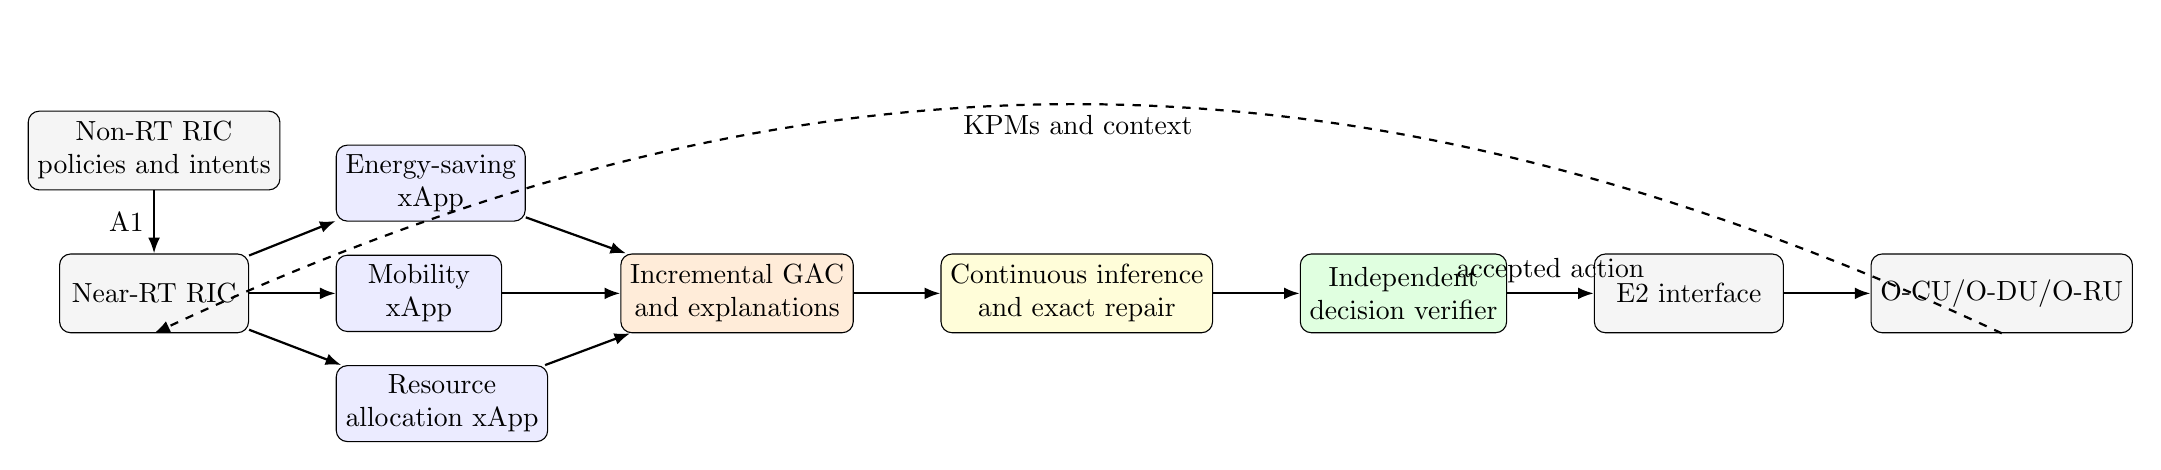
\begin{tikzpicture}[
    node distance=8mm and 11mm,
    block/.style={
        draw,
        rounded corners,
        align=center,
        minimum width=24mm,
        minimum height=10mm,
        fill=gray!8
    },
    app/.style={
        draw,
        rounded corners,
        align=center,
        minimum width=21mm,
        minimum height=9mm,
        fill=blue!8
    },
    prop/.style={
        draw,
        rounded corners,
        align=center,
        minimum width=26mm,
        minimum height=10mm,
        fill=orange!15
    },
    coord/.style={
        draw,
        rounded corners,
        align=center,
        minimum width=27mm,
        minimum height=10mm,
        fill=yellow!15
    },
    verify/.style={
        draw,
        rounded corners,
        align=center,
        minimum width=25mm,
        minimum height=10mm,
        fill=green!12
    },
    arrow/.style={-{Latex[length=2mm]},thick}
]

\node[block] (nonrt) {Non-RT RIC\\policies and intents};
\node[block, below=of nonrt] (near) {Near-RT RIC};

\node[app, right=of near, yshift=14mm] (x1)
{Energy-saving\\xApp};

\node[app, right=of near] (x2)
{Mobility\\xApp};

\node[app, right=of near, yshift=-14mm] (x3)
{Resource\\allocation xApp};

\node[prop, right=15mm of x2] (gac)
{Incremental GAC\\and explanations};

\node[coord, right=of gac] (coord)
{Continuous inference\\and exact repair};

\node[verify, right=of coord] (verifier)
{Independent\\decision verifier};

\node[block, right=of verifier] (e2)
{E2 interface};

\node[block, right=of e2] (ran)
{O-CU/O-DU/O-RU};

\draw[arrow] (nonrt) -- node[left]{A1} (near);

\draw[arrow] (near) -- (x1);
\draw[arrow] (near) -- (x2);
\draw[arrow] (near) -- (x3);

\draw[arrow] (x1) -- (gac);
\draw[arrow] (x2) -- (gac);
\draw[arrow] (x3) -- (gac);

\draw[arrow] (gac) -- (coord);
\draw[arrow] (coord) -- (verifier);
\draw[arrow] (verifier) -- node[above]{accepted action} (e2);
\draw[arrow] (e2) -- (ran);

\draw[arrow,dashed] (ran.south) to[bend right=25]
node[below]{KPMs and context} (near.south);

\end{tikzpicture}
}
\caption{
Position of \method\ in the near-real-time RIC control path.
Generalized arc consistency filters unsupported actions before
continuous coordination. Propagation explanations guide exact repair,
and every final action is independently verified.
}
\label{fig:architecture}
\end{figure*}

\subsection{xApp conflict types}

Let $\mathcal{A}=\{1,\ldots,n\}$ denote the set of active xApp action
variables, $\mathcal{P}$ the set of network control parameters, and
$\mathcal{K}$ the set of monitored KPMs.

A direct conflict occurs when two or more xApps propose incompatible
values for the same parameter. For example, a coverage xApp may
request a transmission-power increase while an interference or
energy-saving xApp requests a decrease.

An indirect conflict occurs when xApps modify different parameters
that influence the same KPM. A load-balancing xApp may modify cell
individual offsets while a mobility xApp modifies handover
thresholds. Both actions affect cell association and load.

An implicit conflict occurs when actions targeting distinct
parameters and KPMs interact through the RAN dynamics. For example,
putting a cell into a low-energy state may reduce energy consumption
but increase mobility failures or violate slice-throughput
requirements.

Direct conflicts can often be verified syntactically. Indirect
conflicts require a registered parameter--KPM dependency model.
Implicit conflicts require a validated impact model, digital twin,
emulator, or conservative operator rule.

\subsection{xApp conflict-management approaches}

Adamczyk and Kliks proposed a conflict-mitigation framework embedded
in the near-real-time RIC, including conflict-detection and
conflict-resolution mechanisms \cite{adamczyk2023conflict}. QACM
formulates resolution as a QoS-aware optimization problem seeking to
satisfy the requirements of multiple xApps \cite{wadud2024qacm}.

PACIFISTA profiles O-RAN applications in a controlled environment and
uses statistical models and hierarchical graphs to characterize
conflicts before deployment \cite{prever2025pacifista}. COMIX
combines conflict management with a network digital twin for
multi-channel power control \cite{giannopoulos2025comix}.
Mobility-driven energy-saving experiments have also been used to
study direct, indirect, and implicit conflicts
\cite{wadud2025mobility}. Closest in spirit to our auditability goal,
XAI4C applies explainable-AI techniques to conflict detection and
mitigation in the near-real-time RIC \cite{varshney2025xai4c}; its
explanations are post-hoc attributions of a learned detector, whereas
the explanations produced here are logical premises replayable against
the registered constraint model and checkable by an independent
verifier.

The present work does not replace prediction, profiling, or digital
twins. It addresses finite-domain reasoning after candidate actions
and conflict relations have been registered.

\subsection{Constraint consistency}

Constraint propagation reduces variable domains by removing values
that cannot participate in locally supported tuples. For binary
constraints, this property is expressed through arc consistency.
For non-binary relations, generalized arc consistency requires each
remaining value to have a support in every incident constraint
\cite{yap2020gac}.

Positive table constraints, such as the allowed relations used in
this paper, can be filtered by generic GAC algorithms or specialized
table-reduction procedures such as STR and STR2
\cite{lecoutre2011str2}.

Local consistency is not a complete decision procedure in general.
A constraint network may be GAC while admitting no global solution.
Nevertheless, propagation can detect some contradictions without
search, remove unsupported values, reduce active relation tables, and
produce structural information for diagnosis and repair.

\subsection{Dynamic CSPs and explanations}

Dynamic constraint satisfaction studies sequences of related CSPs
whose domains or constraints evolve over time. Incremental
arc-consistency algorithms reuse information from preceding problems
instead of recomputing all supports from scratch
\cite{bessiere1991dynamic}.

This setting is relevant to the near-real-time RIC because consecutive
decision epochs commonly differ only in a subset of active xApps,
measurements, policies, domains, or context-dependent relations.

Explanations associate a value removal or contradiction with a set of
constraints and decisions sufficient to justify it. They support
diagnosis, conflict analysis, dynamic retraction, and repair in
constraint programming \cite{gupta2021explanations}.

Propagation and explanations are established constraint-programming
concepts. The contribution of this work is their integration with
dynamic xApp coordination, consistency-filtered continuous inference,
fractional-stall diagnosis, deadline-bounded exact repair, and
independent execution verification.

% ============================================================
\section{Dynamic System and Conflict Model}
\label{sec:model}
% ============================================================

\subsection{Decision epochs and candidate actions}

The near-real-time RIC operates over decision epochs
$t=1,\ldots,T$. At epoch $t$, each active xApp action variable $i$
has a finite base domain

\begin{equation}
D_i^t
=
\left\{
a_{i,1}^t,\ldots,a_{i,d_i}^t
\right\}.
\end{equation}

An action may represent:

\begin{itemize}
    \item accepting or rejecting a control request;
    \item selecting a target cell;
    \item assigning an execution slot;
    \item selecting a discrete transmission-power level;
    \item applying a configured handover offset;
    \item selecting a radio-resource-allocation profile;
    \item executing a registered safe no-operation action.
\end{itemize}

The discrete variable $x_i^t\in D_i^t$ represents the coordinated
action selected for variable $i$. The time index is omitted when a
single decision epoch is considered.

\subsection{Context-dependent conflict relations}

A constraint $c\in\mathcal{C}_t$ has scope
$S_c\subseteq\mathcal{A}_t$ and an allowed relation

\begin{equation}
R_c(\bm{s}_t)
\subseteq
\prod_{i\in S_c}D_i^t,
\end{equation}

where $\bm{s}_t$ denotes the observed and registered network context.

An assignment $\bm{x}^t$ satisfies constraint $c$ if

\begin{equation}
\bm{x}_{S_c}^t
\in
R_c(\bm{s}_t).
\end{equation}

Relations may be binary or higher-order. They can be generated from:

\begin{enumerate}
    \item operator policies;
    \item parameter-ownership declarations;
    \item SLA and QoS thresholds;
    \item validated xApp profiles;
    \item a calibrated simulator or digital twin;
    \item conservative safety rules.
\end{enumerate}

Hard constraints must be satisfied before a decision is executed.
Soft constraints contribute to utility but may be violated at a
specified cost.

\subsection{Dynamic coordination sequence}

The hard coordination model at epoch $t$ is

\begin{equation}
\mathcal{M}_t
=
\left(
\mathcal{A}_t,
\bm{D}_t,
\mathcal{C}_t,
\bm{s}_t
\right),
\end{equation}

where $\bm{D}_t=(D_i^t)_{i\in\mathcal{A}_t}$.

The transition from $\mathcal{M}_{t-1}$ to $\mathcal{M}_t$ may
contain:

\begin{itemize}
    \item activation or deactivation of an xApp;
    \item addition or removal of candidate actions;
    \item addition or removal of a constraint;
    \item restriction or relaxation of a relation;
    \item modification of an SLA threshold;
    \item modification of a parameter--KPM dependency;
    \item updated utility or confidence estimates.
\end{itemize}

The modified variables and constraints are denoted by

\begin{equation}
\Delta_t
=
\Delta_t^{\mathrm{var}}
\cup
\Delta_t^{\mathrm{con}}.
\end{equation}

Restrictive and relaxation updates must be distinguished. After a
restrictive update, previous support information may remain reusable.
After a relation or domain relaxation, a previously removed value may
become supported and must be restored from its current base domain
before propagation is re-established.

\subsection{Utility and temporal stability}

Let $u_i(a_i,\bm{s}_t)$ denote the predicted or measured utility of
selecting action $a_i$ for variable $i$, and let
$\omega_i\geq 0$ denote its operator-defined weight.

The static utility is

\begin{equation}
U(\bm{x},\bm{s}_t)
=
\sum_{i\in\mathcal{A}_t}
\omega_i u_i(x_i,\bm{s}_t)
-
\sum_{q\in\mathcal{Q}_t}
\lambda_q v_q(\bm{x},\bm{s}_t),
\label{eq:static-utility}
\end{equation}

where $v_q$ is a non-negative soft-violation penalty and
$\lambda_q\geq 0$ is its weight.

Let $\bm{x}^{t-1}$ be the previous verified decision. The weighted
action-churn measure is

\begin{equation}
H(\bm{x}^{t},\bm{x}^{t-1})
=
\sum_{i\in\mathcal{A}_t\cap\mathcal{A}_{t-1}}
\kappa_i
\mathbf{1}
\left[
x_i^t\neq x_i^{t-1}
\right],
\label{eq:churn}
\end{equation}

where $\kappa_i\geq 0$ is a reconfiguration cost.

The dynamic utility is

\begin{equation}
U_t^{\mathrm{dyn}}(\bm{x}^{t})
=
U(\bm{x}^{t},\bm{s}_t)
-
\mu
H(\bm{x}^{t},\bm{x}^{t-1}),
\label{eq:dynamic-utility}
\end{equation}

where $\mu\geq 0$ controls the trade-off between instantaneous utility
and temporal stability.

Dwell-time, cooldown, and maximum-change rules are represented as hard
relations when violation is not permitted.

The dynamic finite-domain optimization problem is

\begin{align}
\max_{\bm{x}^{t}}\quad&
U_t^{\mathrm{dyn}}(\bm{x}^{t})
\label{eq:problem-objective}\\
\text{s.t.}\quad&
x_i^t\in D_i^t,
&&i\in\mathcal{A}_t,
\label{eq:problem-domain}\\
&
\bm{x}_{S_c}^t\in R_c(\bm{s}_t),
&&c\in\mathcal{C}_{t,\mathrm{hard}}.
\label{eq:problem-hard}
\end{align}

\subsection{Conflict-hypergraph representation}

We define a heterogeneous dependency graph

\begin{equation}
G_t=(V_t,E_t),
\end{equation}

whose nodes include xApp action variables, control parameters,
constraints, and KPMs. An edge records that:

\begin{itemize}
    \item an xApp controls a parameter;
    \item a parameter influences a KPM;
    \item a constraint contains a variable;
    \item a KPM belongs to an SLA.
\end{itemize}

The constraint scopes additionally induce a hypergraph over the
decision variables. The graph and hypergraph support incremental
queue initialization, explanation visualization, and repair-core
construction.

\subsection{Worked example}
\label{sec:worked-example}

Consider a single cell with three concurrent xApps. A coverage xApp
controls transmission power $x_1\in\{\text{low},\text{med},\text{high}\}$,
an energy-saving xApp controls the cell state
$x_2\in\{\text{sleep},\text{on}\}$, and a mobility xApp controls a
handover offset $x_3\in\{-3,0,+3\}$~dB. Two SLAs apply: a minimum
edge-throughput requirement and a maximum handover-failure rate.

The registered hard relations encode these SLAs as allowed tuples.
The power--state relation $R_{12}$ forbids the joint request
(power increase, sleep) because a sleeping cell cannot raise coverage,
and forbids (low, on) because low power violates edge throughput:

\begin{equation}
R_{12}=
\{(\text{med},\text{on}),(\text{high},\text{on}),
(\text{low},\text{sleep})\}.
\end{equation}

Suppose the coverage and energy-saving xApps simultaneously request
$x_1=\text{high}$ and $x_2=\text{sleep}$. Generalized arc consistency
leaves both values in place: \text{high} is supported by
$(\text{high},\text{on})$ and \text{sleep} by $(\text{low},\text{sleep})$,
so every value retains local support (a direct conflict that GAC alone
cannot resolve). The continuous stage may decode the individually
supported pair $(\text{high},\text{sleep})$, which violates $R_{12}$.
The verifier rejects it; the violated relation $R_{12}$ seeds the
repair core $\mathcal{A}^0=\{x_1,x_2\}$, and exact repair returns a
verified alternative such as $(\text{high},\text{on})$ or, if the
energy SLA dominates, $(\text{low},\text{sleep})$, with $x_3$ fixed to
its decoded value on the boundary. This illustrates the division of
labour: propagation prunes unsupported actions, whereas repair resolves
incompatible combinations of individually supported actions.


\section{The \method\ Framework}
\label{sec:method}

% ============================================================
\subsection{Base and filtered domains}
% ============================================================

At epoch $t$, $D_i^t$ denotes the base domain provided by the xApp
registry and the current context. The propagation stage derives a
filtered domain

\begin{equation}
D_i^{t,*}\subseteq D_i^t.
\end{equation}

Base and filtered domains are stored separately. This separation is
required because a later relation or domain relaxation may restore
support for a previously removed value.

For readability, the time index is omitted in the remainder of this
section whenever a single decision epoch is considered.

% ============================================================
\subsection{Generalized arc consistency}
% ============================================================

Given current domains

\begin{equation}
\bm{D}=(D_1,\ldots,D_n),
\end{equation}

the support set of value $a\in D_i$ in constraint $c$ is

\begin{equation}
\operatorname{Supp}_{c}
(i,a;\bm{D})
=
\left\{
\bm{z}\in R_c(\bm{s}_t):
z_i=a
\land
z_j\in D_j,\;
\forall j\in S_c
\right\}.
\label{eq:support}
\end{equation}

\begin{definition}[Generalized arc consistency]
A hard relation $R_c$ is generalized arc consistent with respect to
$\bm{D}$ if

\begin{equation}
\operatorname{Supp}_{c}(i,a;\bm{D})
\neq\varnothing
\end{equation}

for every $i\in S_c$ and every $a\in D_i$. The hard constraint
network is generalized arc consistent if every hard relation is
generalized arc consistent.
\end{definition}

The revision operator for variable $i$ and constraint $c$ is

\begin{equation}
\operatorname{Revise}_{c,i}(\bm{D}):
\quad
D_i
\leftarrow
\left\{
a\in D_i:
\operatorname{Supp}_{c}(i,a;\bm{D})
\neq\varnothing
\right\}.
\label{eq:revise}
\end{equation}

Revision is repeatedly applied through a propagation queue until no
domain changes. The resulting domain vector is denoted by

\begin{equation}
\bm{D}^{*}
=
\operatorname{GAC}
\left(
\bm{D},
\mathcal{C}_{\mathrm{hard}},
\bm{s}_t
\right).
\label{eq:gac-closure}
\end{equation}

If $D_i^{*}=\varnothing$ for at least one variable, propagation has
detected a domain wipeout. Such a wipeout proves that no feasible
assignment extends the current domains.

The converse does not hold: non-empty GAC domains do not, in general,
prove global feasibility.

% ============================================================
\subsection{Incremental propagation}
% ============================================================

At epoch $t$, the propagation queue is initialized with the
constraints affected by $\Delta_t$ and the constraints sharing an
affected variable.

For a purely restrictive transition, unchanged supports and previous
value deletions can be reused when the premises of those deletions
remain valid.

For a relaxation transition, affected variables are first restored
from their current base domains. Propagation is then re-established
on the affected connected component. This restoration rule prevents
stale deletions from being carried unsoundly across a relaxed context.

For explicit positive-table constraints, the implementation records:

\begin{itemize}
    \item the currently active tuples;
    \item the last known support of each variable--value pair;
    \item the context identifier under which each support was valid;
    \item the explanation associated with each value removal.
\end{itemize}

These structures accelerate propagation but do not alter the GAC
semantics of Equation~\eqref{eq:gac-closure}.

The incremental procedure processes an epoch as follows:

\begin{enumerate}
    \item identify the variables and constraints modified by
    $\Delta_t$;

    \item classify the transition as restrictive, relaxed, mixed, or
    utility-only;

    \item restore affected base-domain values if the transition
    contains a relaxation;

    \item invalidate cached supports whose relation, domain, or
    context identifier has changed;

    \item initialize the propagation queue with the affected
    constraints;

    \item repeatedly revise incident variable domains until the queue
    becomes empty or a domain wipeout occurs;

    \item store the resulting filtered domains, active tuples,
    supports, and explanations for the next epoch.
\end{enumerate}

An implementation may use a generic GAC-Schema algorithm,
STR2-style table reduction, or another positive-table propagator.
The artifact must identify the implemented algorithm. Solver-internal
propagation is not counted as the proposed observable GAC stage unless
its filtered domains, explanations, and timing can be extracted
independently.

% ============================================================
\subsection{Propagation explanations}
% ============================================================

Let $\mathcal{L}$ denote temporary domain restrictions and boundary
decisions. When value $a$ is removed from $D_i$ by constraint $c$, the
propagator records an explanation

\begin{equation}
\mathcal{E}(i,a)
\subseteq
\mathcal{C}_{\mathrm{hard}}
\cup
\mathcal{L}.
\label{eq:value-explanation}
\end{equation}

The explanation contains sufficient premises to establish that every
tuple in $R_c$ assigning $a$ to $x_i$ is incompatible with the current
domains.

For an explicit positive table, define

\begin{equation}
R_c(i=a)
=
\left\{
\bm{z}\in R_c:z_i=a
\right\}.
\end{equation}

If $a$ is unsupported, then each tuple
$\bm{z}\in R_c(i=a)$ contains at least one component value
$z_j\notin D_j$. A valid explanation identifies, for each candidate
support tuple, at least one premise explaining why that tuple is
inactive.

A complete-base-model wipeout proves infeasibility of the unchanged model; exact search cannot recover a feasible solution, and safe fallback requires an explicitly registered emergency model, authorized request retraction, or policy relaxation under a new context identifier. By contrast, boundary-fixed repair wipeout requires only core expansion and unfixing of responsible boundary variables. A domain-wipeout explanation for variable $i$ is obtained by combining
the explanations of all removed values:

\begin{equation}
\mathcal{E}_{\emptyset}(i)
=
\bigcup_{a\in D_i^{\mathrm{base}}}
\mathcal{E}(i,a),
\label{eq:wipeout-explanation}
\end{equation}

where $D_i^{\mathrm{base}}$ denotes the relevant base domain at the
current epoch.

The framework does not require explanations to be
cardinality-minimal. It requires them to be:

\begin{itemize}
    \item logically valid relative to the registered model;
    \item reproducible from the propagation trace;
    \item associated with a context identifier;
    \item auditable by a separately implemented explanation checker.
\end{itemize}

Explanation minimization is treated as an optional optimization and
must not alter correctness.

% ============================================================
\subsection{Consistency-filtered continuous lifting}
% ============================================================

If propagation terminates without a domain wipeout, each discrete
variable is lifted over its filtered domain:

\begin{equation}
\bm{p}_i
\in
\Delta(D_i^{*})
=
\left\{
\bm{p}\in\mathbb{R}_{+}^{|D_i^{*}|}:
\sum_{a\in D_i^{*}}p(a)=1
\right\}.
\end{equation}

If xApp confidence values are available, they are projected onto the
filtered domain:

\begin{equation}
p_i^{0}(a)
=
\frac{\overline{p}_i(a)}
{\displaystyle
\sum_{b\in D_i^{*}}\overline{p}_i(b)},
\qquad
a\in D_i^{*},
\label{eq:projected-initialization}
\end{equation}

where $\overline{p}_i$ is the confidence distribution over the base
domain.

If

\begin{equation}
\sum_{b\in D_i^{*}}\overline{p}_i(b)=0,
\end{equation}

the marginal is initialized uniformly on $D_i^{*}$. When no
confidence information is available, a uniform initialization with
documented seeded noise is used.

Removed values have zero probability and do not participate in the
continuous update. The joint state is

\begin{equation}
\bm{p}
=
(\bm{p}_1,\ldots,\bm{p}_n)
\in
\prod_{i=1}^{n}\Delta(D_i^{*}).
\end{equation}

% ============================================================
\subsection{Active relation tables}
% ============================================================

After propagation, the active part of relation $c$ is

\begin{equation}
R_c^{*}
=
\left\{
\bm{z}\in R_c(\bm{s}_t):
z_j\in D_j^{*},
\;
\forall j\in S_c
\right\}.
\label{eq:active-relation}
\end{equation}

For a non-empty GAC model, every value in every filtered domain has at
least one support in each incident active relation.

The use of $R_c^{*}$ avoids assigning continuous mass to tuples that
have already been invalidated by sound domain filtering.

% ============================================================
\subsection{Relation-conditioned messages}
% ============================================================

For each active tuple $\bm{z}\in R_c^{*}$, define

\begin{equation}
w_c(\bm{z};\bm{p})
=
\exp\left[
\frac{1}{\tau}
\left(
\sum_{j\in S_c}
\log\max\{p_j(z_j),\varepsilon\}
+
\gamma_c u_c(\bm{z})
\right)
\right],
\label{eq:tuple-weight}
\end{equation}

where:

\begin{itemize}
    \item $\tau>0$ is a temperature;
    \item $\varepsilon>0$ prevents logarithms of zero;
    \item $u_c$ is an optional local utility;
    \item $\gamma_c$ controls its influence.
\end{itemize}

The relation-conditioned message from constraint $c$ to variable $i$
is

\begin{equation}
\pi_{c\rightarrow i}(a)
=
\frac{
\displaystyle
\sum_{\substack{\bm{z}\in R_c^{*}\\z_i=a}}
w_c(\bm{z};\bm{p})
}{
\displaystyle
\sum_{\bm{z}\in R_c^{*}}
w_c(\bm{z};\bm{p})
}.
\label{eq:message}
\end{equation}

Log-sum-exp normalization is used in the implementation to prevent
numerical underflow.

Because GAC was established before continuous inference, the
numerator of Equation~\eqref{eq:message} has at least one structural
support for every $a\in D_i^{*}$. A numerically negligible message
must therefore be distinguished from the absence of a relational
support.

% ============================================================
\subsection{Geometric consensus}
% ============================================================

Let $\mathcal{C}_i$ denote the set of hard constraints incident to
variable $i$. For $\mathcal{C}_i\neq\varnothing$, the log-domain
consensus is

\begin{equation}
\ell_i(a)
=
\alpha
\log\max\{p_i(a),\varepsilon\}
+
\sum_{c\in\mathcal{C}_i}
\eta_{c,i}
\log\max\{
\pi_{c\rightarrow i}(a),\varepsilon
\},
\label{eq:consensus}
\end{equation}

where $\alpha\geq 0$ is an inertia parameter and

\begin{equation}
\eta_{c,i}>0,
\qquad
\sum_{c\in\mathcal{C}_i}\eta_{c,i}=1.
\end{equation}

For a variable with no incident hard constraint, the update retains
its current marginal or uses a separately documented utility-based
update.

The normalized consensus marginal is

\begin{equation}
\widehat{p}_i(a)
=
\frac{\exp(\ell_i(a))}
{\displaystyle
\sum_{b\in D_i^{*}}
\exp(\ell_i(b))}.
\end{equation}

A polarization step is applied:

\begin{equation}
q_i(a)
=
\frac{
\widehat{p}_i(a)^{\beta}
}{
\displaystyle
\sum_{b\in D_i^{*}}
\widehat{p}_i(b)^{\beta}
},
\qquad
\beta\geq 1.
\label{eq:polarization}
\end{equation}

Finally, clipping and renormalization give

\begin{equation}
p_i^{+}(a)
=
\frac{
\max\{q_i(a),\varepsilon\}
}{
\displaystyle
\sum_{b\in D_i^{*}}
\max\{q_i(b),\varepsilon\}
}.
\label{eq:clipping}
\end{equation}

Equations~\eqref{eq:tuple-weight}--\eqref{eq:clipping} define the
continuous update map

\begin{equation}
T:\bm{p}\mapsto\bm{p}^{+}.
\end{equation}

No claim is made that $T$ is an exact ascent or descent step for a
global optimization objective.

\begin{remark}[Relation to message passing]
Equations~\eqref{eq:tuple-weight}--\eqref{eq:message} resemble the
sum-product messages of loopy belief propagation and mean-field
inference on a factor graph
\cite{yedidia2003understanding,wainwright2005map,bayati2011bmatching}.
Two deliberate differences must be stated. First, the tuple weight
$w_c(\bm{z};\bm{p})$ in Equation~\eqref{eq:tuple-weight} includes the
factor $p_i(z_i)$ of the receiving variable itself, so
$\pi_{c\rightarrow i}$ is not a cavity (extrinsic) message in the sense
of standard belief propagation. Second, the geometric consensus in
Equation~\eqref{eq:consensus}, the polarization exponent
$\beta\geq 1$, and the clipping in Equation~\eqref{eq:clipping} are
introduced to drive the marginals towards near-integral consensus on
the filtered domains rather than to compute exact marginals of a
probabilistic model. The update is therefore a heuristic
relation-conditioned consensus, not exact belief propagation, not
mean-field free-energy minimization, and not a guaranteed optimizer of
any global objective. Its role in \method\ is purely to expose an
integral candidate and diagnostic residual for the verifier and
repair stages; soundness is provided by the independent verifier and
by exact repair, never by the continuous map.
\end{remark}

% ============================================================
\subsection{Decoding}
% ============================================================

The discrete candidate is obtained by deterministic decoding:

\begin{equation}
\widehat{x}_i
=
\arg\max_{a\in D_i^{*}}p_i(a).
\label{eq:decode}
\end{equation}

Ties are broken according to a fixed documented order. The decoded
candidate is not considered executable until it has passed the
independent verifier.

% ============================================================
\subsection{Coordination diagnostics}
% ============================================================

The update residual is

\begin{equation}
\rho(\bm{p})
=
\max_{i\in\mathcal{A}}
\left\|
T_i(\bm{p})-\bm{p}_i
\right\|_1.
\label{eq:residual}
\end{equation}

Let

\begin{equation}
\mathcal{A}_{>1}
=
\left\{
i\in\mathcal{A}:|D_i^{*}|>1
\right\}.
\end{equation}

If $\mathcal{A}_{>1}\neq\varnothing$, the domain-filtered
fractionality score is

\begin{equation}
\phi(\bm{p})
=
\frac{1}{|\mathcal{A}_{>1}|}
\sum_{i\in\mathcal{A}_{>1}}
\left(
1-\max_{a\in D_i^{*}}p_i(a)
\right).
\label{eq:fractionality}
\end{equation}

If $\mathcal{A}_{>1}=\varnothing$, $\phi(\bm{p})$ is defined as zero.

The number of violated hard relations is

\begin{equation}
V(\widehat{\bm{x}})
=
\sum_{c\in\mathcal{C}_{\mathrm{hard}}}
\mathbf{1}
\left[
\widehat{\bm{x}}_{S_c}
\notin R_c(\bm{s}_t)
\right].
\label{eq:violations}
\end{equation}

\begin{definition}[Propagation contradiction]
A propagation contradiction occurs when

\begin{equation}
\exists i\in\mathcal{A},
\qquad
D_i^{*}=\varnothing.
\end{equation}

The associated wipeout explanation identifies a sufficient set of
constraints and temporary restrictions responsible for the detected
contradiction.
\end{definition}

\begin{definition}[Operational fractional stall]
A non-empty propagated state is classified as an operational
fractional stall if

\begin{equation}
\rho(\bm{p})\leq\delta_{\rho},
\qquad
\phi(\bm{p})\geq\delta_{\phi},
\qquad
V(\widehat{\bm{x}})>0.
\end{equation}
\end{definition}

\begin{definition}[Invalid non-stalled decode]
An invalid non-stalled decode occurs when

\begin{equation}
V(\widehat{\bm{x}})>0
\end{equation}

but at least one numerical stall condition is not satisfied.
\end{definition}

A numerical stall is not presented as proof of the exact equality

\begin{equation}
T(\bm{p})=\bm{p}.
\end{equation}

It is an operational diagnosis based on a finite numerical tolerance.

Both invalid stalls and invalid non-stalled decodes trigger exact
repair. Their distinction is retained for analysis rather than
decision soundness.

% ============================================================
\subsection{Explanation-guided exact repair}
\label{sec:repair}
% ============================================================

When the decoded candidate is invalid, the initial conflict set is

\begin{equation}
\mathcal{C}^{0}
=
\left\{
c\in\mathcal{C}_{\mathrm{hard}}:
\widehat{\bm{x}}_{S_c}
\notin R_c(\bm{s}_t)
\right\}.
\label{eq:initial-conflicts}
\end{equation}

The initial variable core is

\begin{equation}
\mathcal{A}^{0}
=
\bigcup_{c\in\mathcal{C}^{0}}S_c.
\label{eq:initial-core}
\end{equation}

At repair iteration $r$, variables outside the core are temporarily
fixed to their decoded values:

\begin{equation}
D_j^{(r)}
=
\{\widehat{x}_j\},
\qquad
j\notin\mathcal{A}^{r}.
\label{eq:boundary-fixing}
\end{equation}

Variables inside the core retain their filtered domains:

\begin{equation}
D_i^{(r)}
=
D_i^{*},
\qquad
i\in\mathcal{A}^{r}.
\label{eq:core-domain}
\end{equation}

GAC is first enforced on the induced repair model.

If propagation produces a domain wipeout, let
$\mathcal{E}_{\emptyset}^{r}$ denote its explanation. The next
constraint and variable cores are

\begin{align}
\mathcal{C}^{r+1}
&=
\mathcal{C}^{r}
\cup
\left(
\mathcal{E}_{\emptyset}^{r}
\cap
\mathcal{C}_{\mathrm{hard}}
\right),
\label{eq:constraint-expansion}\\
\mathcal A^{r+1} = \mathcal A^r \cup \operatorname{VarLit}(\mathcal E_\emptyset^r) \cup \bigcup_{c\in\mathcal C^{r+1}}S_c.
\label{eq:variable-expansion}
\end{align}

If propagation reaches non-empty domains, the induced subproblem is
passed to an exact solver.

If the exact solver finds a feasible assignment, the candidate is
sent to the independent verifier.

If the local subproblem is infeasible because of fixed boundary
decisions, the core is expanded using an auditable solver conflict
explanation when available.

If the solver adapter exposes no usable conflict explanation, the
framework adds constraints adjacent to the current explanation
frontier according to a deterministic documented rule. This fallback
expansion is distinguished experimentally from explanation-guided
expansion.

\paragraph{Explanation and repair implementation.}
An explanation literal is a pair recording either a hard relation
$c\in\mathcal{C}_{\mathrm{hard}}$ or a temporary domain restriction
$(\,i,a\,)\in\mathcal{L}$ that participated in a removal. The set
$\mathcal{L}$ therefore contains the boundary decisions
$x_j=\widehat{x}_j$ imposed by Equation~\eqref{eq:boundary-fixing}.
The operator $\operatorname{VarLit}(\mathcal{E})$ returns the variables
mentioned by the literals of $\mathcal{E}$, i.e. the removed variables
in $\mathcal{L}$ together with the scope variables of the constraints
in $\mathcal{E}\cap\mathcal{C}_{\mathrm{hard}}$; it is used in
Equation~\eqref{eq:variable-expansion} to grow the variable core.
In the implementation, the repair subproblem is encoded for
\cpsat\ with the fixed boundary values expressed as unit-domain
\texttt{AddAllowedAssignments} constraints (assumption-style literals),
so that an unsatisfiable core returned by the solver identifies the
subset of boundary fixings responsible for local infeasibility. When
the adapter exposes such a core, the responsible boundary variables are
unfixed and added to $\mathcal{A}^{r+1}$; otherwise the deterministic
frontier rule above is applied. Explanations are not required to be
cardinality-minimal: they are validated by the independent checker,
which replays the stated premises, restricts the stated domains, and
verifies that every tuple supporting the pruned value is disabled.
The evaluation reports, for each repair, the initial and final core
sizes, the number of expansions, and whether full-scope escalation was
required, so that explanation-guided localization can be separated from
fallback expansion.

The repair process terminates when:

\begin{enumerate}
    \item a verified repaired decision is found;
    \item the complete variable set has been included;
    \item the repair deadline is reached;
    \item a registered safe fallback must be applied.
\end{enumerate}

The repair objective is lexicographic:

\begin{enumerate}
    \item satisfy every registered hard relation;
    \item minimize weighted reconfiguration relative to the previous
    verified decision;
    \item minimize deviation from the continuous decode;
    \item maximize the static utility $U(\bm{x},\bm{s}_t)$ of
    Equation~\eqref{eq:static-utility}.
\end{enumerate}

The final level uses the \emph{static} utility rather than the dynamic
utility $U_t^{\mathrm{dyn}}$: temporal stability is already enforced
lexicographically by level~2 through $H_{\mathrm{prev}}$, so reusing
$U_t^{\mathrm{dyn}}$ (which itself subtracts $\mu H$) would penalize
reconfiguration a second time. Operators who prefer a single scalar
trade-off may instead drop level~2 and optimize $U_t^{\mathrm{dyn}}$
directly; the two formulations are reported separately in the
artifact.

The two change criteria are

\begin{align}
H_{\mathrm{prev}}(\bm{x})
&=
\sum_i
\kappa_i
\mathbf{1}
[x_i\neq x_i^{t-1}],
\label{eq:previous-distance}\\
H_{\mathrm{decode}}(\bm{x})
&=
\sum_i
\zeta_i
\mathbf{1}
[x_i\neq\widehat{x}_i],
\label{eq:decode-distance}
\end{align}

where $\zeta_i\geq 0$ is the cost of changing the decoded action.

The objective ordering is fixed before evaluation and reported in the
artifact. If no previous verified value exists for a newly activated
variable, that variable contributes zero to
$H_{\mathrm{prev}}$ or uses an explicitly documented initialization
cost.

% ============================================================
\subsection{Safe fallback}
% ============================================================

If repair cannot produce a verified action before the deadline,
\method\ executes a registered safe policy. Depending on the
scenario, this policy may:

\begin{itemize}
    \item reject the conflicting requests;
    \item retain the previous verified configuration;
    \item execute a safe no-operation action;
    \item delegate to a conservative operator rule.
\end{itemize}

A fallback must be represented explicitly in the current action model.
It must satisfy the current domains and hard relations and must pass
the same independent verifier as an optimized action.

Retaining the previous configuration is not automatically safe when
the context or hard relations have changed. The previous decision is
therefore reverified under the current context before reuse.

% ============================================================
\subsection{Independent verifier}
% ============================================================

The verifier is implemented separately from propagation, continuous
inference, explanation construction, and exact repair. It receives:

\begin{itemize}
    \item the current context identifier;
    \item the selected actions;
    \item the current base domains;
    \item the registered hard relations;
    \item the applicable SLA thresholds.
\end{itemize}

The accepted-decision set is

\begin{equation}
\mathcal{F}(\bm{s}_t)
=
\left\{
\bm{x}:
x_i\in D_i,
\;
\bm{x}_{S_c}\in R_c(\bm{s}_t),
\;
\forall c\in\mathcal{C}_{\mathrm{hard}}
\right\}.
\label{eq:feasible-set}
\end{equation}

\begin{proposition}[Decision soundness]
If \method\ forwards an action $\bm{x}$ to the E2 interface, then

\begin{equation}
\bm{x}\in\mathcal{F}(\bm{s}_t)
\end{equation}

relative to the registered domains, relations, context, and verifier
semantics.
\end{proposition}

\begin{proof}
The framework forwards a candidate only if the independent verifier
accepts it. The verifier checks domain membership and every
registered hard relation directly. Therefore, every forwarded
candidate belongs to $\mathcal{F}(\bm{s}_t)$.
\end{proof}

This proposition concerns decision soundness relative to the
registered model. It does not prove that the model perfectly
represents the physical RAN.

% ============================================================
\subsection{End-to-end decision procedure}
% ============================================================

At each decision epoch, \method\ executes the following procedure:

\begin{enumerate}
    \item build or update the dynamic model $\mathcal{M}_t$;

    \item classify $\Delta_t$ and restore affected values when the
    transition contains a relaxation;

    \item enforce incremental GAC;

    \item if propagation produces a domain wipeout, record its
    explanation and attempt explanation-guided exact recovery or
    execute a verified fallback;

    \item otherwise, project xApp confidence values onto the filtered
    domains;

    \item execute relation-conditioned continuous inference until a
    stopping condition is reached;

    \item decode the marginals deterministically;

    \item independently test the decoded candidate;

    \item if the candidate is valid, execute it;

    \item otherwise, diagnose the state and run explanation-guided
    exact repair;

    \item progressively expand the repair core when required;

    \item escalate to full-scope CP-SAT if the local repair is
    unsuccessful and the remaining deadline permits;

    \item send only a verifier-accepted optimized or fallback decision
    to the E2 interface.
\end{enumerate}

Every stage records its own status, latency, context identifier, and
witness. This separation allows propagation, repair, and verification
failures to be audited independently.

% ============================================================
\subsection{Algorithmic summary}
\label{sec:algorithms}
% ============================================================

Algorithms~\ref{alg:incgac}--\ref{alg:verify} summarize the four
components whose interaction defines \method: incremental GAC with
restoration after relaxation, relation-conditioned continuous
inference, explanation-guided repair-core expansion, and independent
verification with fallback selection.

\begin{algorithm}[t]
\caption{Incremental GAC with restoration after relaxation}
\label{alg:incgac}
\small
\algin{warm domains $\bm{D}^{*}_{t-1}$, active tables, change set $\Delta_t$}
\algout{filtered domains $\bm{D}^{*}_t$ or \textsc{wipeout}}
\begin{algsteps}
\item classify $\Delta_t$ as restrictive, relaxed, mixed, or utility-only
\item \textbf{if} $\Delta_t$ contains a relaxation \textbf{then} restore
the affected constraint-graph component to its base domains and current
allowed tuples
\item apply restrictive deletions directly to $\bm{D}^{*}_{t-1}$
\item seed the worklist with constraints incident to changed variables
and relations
\item \textbf{while} worklist non-empty: pop $c$, revise every
$i\in S_c$; if some $D_i^{*}=\varnothing$ \textbf{return}
\textsc{wipeout}; re-queue constraints incident to a shrunk domain
\item \textbf{return} $\bm{D}^{*}_t$
\end{algsteps}
\end{algorithm}

\begin{algorithm}[t]
\caption{Relation-conditioned continuous inference}
\label{alg:continuous}
\small
\algin{filtered domains $\bm{D}^{*}$, active tables $R_c^{*}$}
\algout{decoded $\widehat{\bm{x}}$, residual $\rho$, fractionality $\phi$}
\begin{algsteps}
\item initialize $\bm{p}$ from projected confidences, or uniform with
seeded noise
\item \textbf{repeat} until $\rho\le\delta_\rho$ or iteration limit:
\item \quad for each $c$ and $i\in S_c$, compute $\pi_{c\rightarrow i}$
(Eq.~\eqref{eq:message})
\item \quad update $\bm{p}$ by geometric consensus, polarization,
clipping (Eqs.~\eqref{eq:consensus}--\eqref{eq:clipping})
\item \quad update residual $\rho$ and fractionality $\phi$
\item $\widehat{x}_i\leftarrow\arg\max_{a}p_i(a)$ with fixed tie-break
\item \textbf{return} $\widehat{\bm{x}},\rho,\phi$
\end{algsteps}
\end{algorithm}

\begin{algorithm}[t]
\caption{Explanation-guided repair-core expansion}
\label{alg:repair}
\small
\algin{decoded $\widehat{\bm{x}}$, hard model, deadline}
\algout{verified repaired decision, or \textsc{escalate}/\textsc{fallback}}
\begin{algsteps}
\item $\mathcal{C}^0\leftarrow$ violated relations;
$\mathcal{A}^0\leftarrow\bigcup_{c\in\mathcal{C}^0}S_c$
\item \textbf{repeat} until the deadline or $\mathcal{A}^r=\mathcal{A}$:
\item \quad fix boundary variables $j\notin\mathcal{A}^r$ to
$\widehat{x}_j$ (Eq.~\eqref{eq:boundary-fixing})
\item \quad solve the induced subproblem with \cpsat
\item \quad \textbf{if} solved and the verifier accepts the full
assignment \textbf{then return} it
\item \quad expand $\mathcal{A}^{r+1}$ using the solver core or
explanation frontier (Eq.~\eqref{eq:variable-expansion})
\item \textbf{return} \textsc{escalate} to full scope, else
\textsc{fallback}
\end{algsteps}
\end{algorithm}

\begin{algorithm}[t]
\caption{Independent verification and fallback selection}
\label{alg:verify}
\small
\algin{candidate $\bm{x}$, base domains, hard relations, context}
\algout{forwarded decision or blocked}
\begin{algsteps}
\item \textbf{if} $x_i\in D_i\ \forall i$ and
$\bm{x}_{S_c}\in R_c\ \forall c$ \textbf{then return} forward $\bm{x}$
\item \textbf{for} each registered fallback $\bm{f}$ in priority order:
if $\bm{f}$ passes the same check under the current context,
\textbf{return} forward $\bm{f}$
\item \textbf{return} blocked (no verified action)
\end{algsteps}
\end{algorithm}

% ============================================================
\section{Consistency and Fractional-Stall Analysis}
\label{sec:analysis}
% ============================================================

\subsection{Soundness of consistency filtering}

\begin{proposition}[Solution preservation]
Let $\bm{D}^{*}$ be obtained by repeatedly applying the revision
operator in Equation~\eqref{eq:revise}. For every globally feasible
assignment $\bm{x}\in\mathcal{F}(\bm{s}_t)$,

\begin{equation}
x_i\in D_i^{*},
\qquad
\forall i\in\mathcal{A}.
\end{equation}

Consequently, GAC filtering does not remove any value used by a
globally feasible assignment.
\end{proposition}

\begin{proof}
Consider one revision of variable $i$ by constraint $c$. A value
$a\in D_i$ is removed only when it has no support in $R_c$ under the
current domains.

Assume that a globally feasible assignment $\bm{x}$ uses $x_i=a$.
Because $\bm{x}$ satisfies $c$, the tuple $\bm{x}_{S_c}$ belongs to
$R_c$ and supports $a$, provided that its component values remain in
their domains.

Initially, every component of $\bm{x}$ belongs to its base domain.
By induction over the sequence of revision operations, no component
of $\bm{x}$ can be the first component removed: the remaining
components of $\bm{x}_{S_c}$ would provide a support for it.
Therefore, every component of every globally feasible assignment
remains in the final filtered domains.
\end{proof}

\begin{remark}[Local versus global consistency]
Non-empty GAC domains are not a certificate of global feasibility for
an arbitrary constraint hypergraph. GAC establishes support in each
incident relation separately. Exact search may still be required to
determine whether the local supports can be combined into one global
assignment.
\end{remark}

% ============================================================
\subsection{Sound projection onto filtered domains}
% ============================================================

\begin{proposition}[Filtered-marginal support]
Assume that propagation terminates with non-empty filtered domains.
After the projection in
Equation~\eqref{eq:projected-initialization}, every value outside
$D_i^{*}$ has probability zero, and every positive-probability value
belongs to the GAC-filtered domain.
\end{proposition}

\begin{proof}
The projected marginal is defined only for values in $D_i^{*}$ and is
normalized over that set. Values outside $D_i^{*}$ are excluded and
assigned probability zero by construction.
\end{proof}

This property does not imply that a decoded combination is globally
feasible. It establishes only that continuous inference does not
reintroduce values already removed by sound propagation.

% ============================================================
\subsection{Illustrative arbitration motif}
% ============================================================

Consider two xApp requests that must be assigned to different
execution slots. Let

\begin{equation}
D_1=D_2=\{0,1\}
\end{equation}

and

\begin{equation}
R_{\neq}
=
\{(0,1),(1,0)\}.
\end{equation}

Write the marginals as

\begin{equation}
\bm{p}_1=(s,1-s),
\qquad
\bm{p}_2=(t,1-t).
\end{equation}

At $\tau=1$, $\beta=1$, $\alpha=0$, $\varepsilon=10^{-6}$, without clipping or local
utility, the update is

\begin{align}
s^{+}
&=
\frac{s(1-t)}
{s(1-t)+(1-s)t},
\label{eq:s-update}\\
t^{+}
&=
\frac{t(1-s)}
{t(1-s)+(1-t)s}.
\label{eq:t-update}
\end{align}

\begin{proposition}[Fractional arbitration point]
The interior fixed point of
Equations~\eqref{eq:s-update}--\eqref{eq:t-update} is

\begin{equation}
(s,t)
=
\left(
\frac{1}{2},
\frac{1}{2}
\right).
\end{equation}

The Jacobian at this point is

\begin{equation}
J
=
\begin{bmatrix}
1 & -1\\
-1 & 1
\end{bmatrix},
\end{equation}

with eigenvalues $0$ and $2$. The point is therefore a saddle.
Under identical per-variable lexicographic tie-breaking on identical
domain orderings, both variables decode to the same slot and violate
$R_{\neq}$.
\end{proposition}

\begin{remark}[Instability and seeded noise]
Because the non-zero eigenvalue of $J$ equals $2>1$, the symmetric
point $(1/2,1/2)$ is linearly unstable: any asymmetric perturbation is
amplified by the update. The documented seeded-noise initialization of
Section~\ref{sec:method} exploits exactly this instability, so that a
variable-aware tie-break or a small asymmetric initialization moves the
state away from the symmetric point towards a valid corner such as
$(x_1,x_2)=(0,1)$. The stall is therefore a measure-zero worst case
under exact symmetry; the operational-stall diagnosis and exact repair
guarantee a verified decision even when finite-precision iteration
lingers near the symmetric point.
\end{remark}

\begin{proof}
At an interior fixed point,
Equation~\eqref{eq:s-update} requires

\begin{equation}
s(1-t)+(1-s)t=1-t.
\end{equation}

Symmetrically,

\begin{equation}
t(1-s)+(1-t)s=1-s.
\end{equation}

Subtracting the two equations gives $s=t$. Substitution yields

\begin{equation}
2s^2-3s+1=0.
\end{equation}

The interior solution is $s=1/2$. Differentiating the update map at
$(1/2,1/2)$ gives the stated Jacobian. Its eigenvalues are $0$ and
$2$.
\end{proof}

% ============================================================
\subsection{GAC does not eliminate the symmetric stall}
% ============================================================

\begin{proposition}[Persistence of a symmetric stall after GAC]
The different-slot instance above is generalized arc consistent, but
GAC removes no value and does not prevent invalid deterministic
decoding of the uniform continuous state.
\end{proposition}

\begin{proof}
Value $0$ of $x_1$ is supported by $x_2=1$, and value $1$ of $x_1$ is
supported by $x_2=0$. The same argument holds symmetrically for $x_2$.
The relation is therefore GAC.

At the uniform continuous state, both actions have equal probability
for both variables. Identical deterministic tie-breaking selects the
same action for both variables, producing either $(0,0)$ or $(1,1)$.
Neither tuple belongs to $R_{\neq}$.
\end{proof}

This result establishes that propagation and exact repair address
different failure modes. Propagation removes unsupported individual
actions. Exact repair resolves incompatible combinations of actions
that are individually supported.

The result also prevents an incorrect interpretation of GAC as a
complete replacement for the continuous-stage verifier. Local support
and valid global decoding are distinct properties.

% ============================================================
\subsection{Conditional completeness of escalating repair}
% ============================================================

\begin{proposition}[Conditional completeness]
Assume that:

\begin{enumerate}
    \item the repair core is eventually expanded to all variables;
    \item the full-scope exact solver is complete;
    \item the solver time limit is not reached.
\end{enumerate}

Then the repair procedure returns a feasible assignment if and only if
the registered hard constraint model is feasible.
\end{proposition}

\begin{proof}
When the repair core contains every variable, no variable is fixed to
an external decoded boundary value. The repair model is then identical
to the complete hard constraint model. The result follows from the
assumed completeness of the exact solver.
\end{proof}

\begin{remark}
A repair restricted to a proper subset of variables is not globally
complete. Its infeasibility may be caused by fixed boundary decisions
even when the complete model is feasible. Consequently, local
infeasibility must not be reported as global model infeasibility.
\end{remark}

% ============================================================
\subsection{Explanation-guided expansion}
% ============================================================

\begin{proposition}[Monotone repair-core expansion]
The repair sequence satisfies

\begin{equation}
\mathcal{A}^{0}
\subseteq
\mathcal{A}^{1}
\subseteq
\cdots
\subseteq
\mathcal{A}.
\end{equation}

If each unsuccessful non-full repair adds at least one previously
absent variable, then the procedure reaches the full variable set
after at most

\begin{equation}
|\mathcal{A}|-|\mathcal{A}^{0}|
\end{equation}

strict expansions.
\end{proposition}

\begin{proof}
Equation~\eqref{eq:variable-expansion} constructs
$\mathcal{A}^{r+1}$ as the union of $\mathcal{A}^{r}$ and additional
constraint scopes. Therefore,
$\mathcal{A}^{r}\subseteq\mathcal{A}^{r+1}$.

If each unsuccessful non-full iteration adds at least one new
variable, at most
$|\mathcal{A}|-|\mathcal{A}^{0}|$ such additions are possible before
the complete variable set is reached.
\end{proof}

This proposition concerns termination of expansion, not runtime
within a real-time deadline. Each propagation or solving call may
still be computationally expensive.

% ============================================================
\subsection{Dynamic restoration requirement}
% ============================================================

\begin{proposition}[Necessity of restoration after relaxation]
Suppose a value $a$ is removed at epoch $t-1$ because it has no
support in relation $R_c(\bm{s}_{t-1})$. If the relation is relaxed at
epoch $t$, retaining the deletion without re-evaluating the base value
may remove a value that belongs to a feasible assignment of
$\mathcal{M}_t$.
\end{proposition}

\begin{proof}
A relation relaxation may introduce a tuple
$\bm{z}\in R_c(\bm{s}_t)$ with $z_i=a$ that was absent from
$R_c(\bm{s}_{t-1})$. If the remaining tuple components are compatible
with the current domains, $\bm{z}$ is a new support for $a$.
Therefore, the previous no-support explanation is no longer valid.
Keeping $a$ deleted without restoration and re-evaluation may exclude
a current feasible assignment.
\end{proof}

This result justifies maintaining base domains separately from
filtered domains and invalidating explanations whose context premises
have changed.

% ============================================================
\subsection{Computational cost}
% ============================================================

For explicit positive-table constraints, one complete table scan has
the conservative cost

\begin{equation}
O\left(
\sum_{c\in\mathcal{C}_{\mathrm{hard}}}
|R_c|\,|S_c|
\right).
\label{eq:gac-cost}
\end{equation}

Actual propagation cost depends on:

\begin{itemize}
    \item support caching;
    \item tuple invalidation;
    \item incremental queue scheduling;
    \item the number of removed values;
    \item relation arity;
    \item explanation construction.
\end{itemize}

After propagation, one explicit continuous epoch requires

\begin{equation}
O\left(
\sum_{c\in\mathcal{C}}
|R_c^{*}|\,|S_c|
\right).
\label{eq:continuous-cost}
\end{equation}

Propagation benefits continuous inference only when the reduction in
active values, active tuples, continuous iterations, or repair work
offsets the propagation overhead.

Exact repair remains exponential in the worst case. Consequently, the
evaluation must report:

\begin{itemize}
    \item propagation time;
    \item tuple-support inspections;
    \item explanation size and construction time;
    \item number of repair-core expansions;
    \item initial and final core sizes;
    \item local and full-scope solver times;
    \item total decision latency;
    \item deadline compliance.
\end{itemize}

The continuous stage is not assumed to improve runtime merely because
it exposes fractional states. Its value relative to GAC followed
directly by CP-SAT is an experimental question.


\section{Experimental Methodology}
\label{sec:experiments}

% ============================================================
\subsection{Research questions}
% ============================================================

The evaluation addresses the following research questions.

\begin{description}

    \item[RQ1:]
    How many unsupported action values and inactive relation tuples
    are removed by incremental GAC?

    \item[RQ2:]
    How much propagation work is reused between consecutive decision
    epochs, and what is the cost of correctly processing relation
    relaxations?

    \item[RQ3:]
    Does consistency filtering reduce continuous iterations,
    fractional-stall frequency, invalid decoding, or repair frequency?

    \item[RQ4:]
    Does explanation-guided expansion produce smaller or faster
    repair cores than fixed-radius graph expansion?

    \item[RQ5:]
    Under which problem sizes, change rates, and deadlines does the
    proposed architecture outperform complete CP-SAT and warm-started
    CP-SAT, in both cold-start and sequential (amortized) settings?

    \item[RQ6:]
    What is the effect of temporal stability on action churn, network
    utility, throughput, energy, load balance, and mobility?

    \item[RQ7:]
    How reliably do propagation explanations identify unsupported
    actions, boundary-induced local infeasibility, and contradictory
    contexts?

    \item[RQ8:]
    Does the independent verifier agree with an exhaustive oracle and
    with a second implementation that shares no evaluation code, under
    exhaustive, randomized, and adversarially mutated inputs?

\end{description}

% ============================================================
\subsection{Experimental platform}
% ============================================================

The experiments use a Python-based O-RAN coordination simulator. The
scenario, dynamic, ablation, and temporal campaigns were executed on
the reference host recorded in the primary manifest; the cold-start
frontier, amortized sequential, literature-baseline, and
verifier-validation campaigns were executed in a documented secondary
Linux environment recorded in a secondary manifest. All paired
comparisons are within-environment. The platform contains:

\begin{itemize}
    \item a dynamic finite-domain instance generator;
    \item an observable GAC propagator for positive table relations;
    \item an incremental support cache;
    \item a propagation-explanation recorder and checker;
    \item the continuous relation-conditioned coordinator;
    \item an OR-Tools CP-SAT adapter
    \cite{ortools,perron2023cpsat};
    \item a progressively expanding exact-repair adapter;
    \item an independent decision verifier;
    \item a pseudo-physical network model.
\end{itemize}

The pseudo-physical model maps coordinated actions to transmission
power, radio-resource fractions, handover offsets, cell sleep states,
and user association. It derives SINR, throughput, energy, fairness,
cell-load, and handover-failure indicators.

The released artifact must report:

\begin{itemize}
    \item the Python and OR-Tools versions;
    \item the GAC implementation and its support structures;
    \item the explanation format and explanation checker;
    \item the continuous-update parameters;
    \item the exact-solver parameters and time limits;
    \item all scenario configurations;
    \item the instance and trace seed hierarchy;
    \item the processor and memory of the evaluation host;
    \item the raw per-epoch logs;
    \item the scripts used to generate every table and figure.
\end{itemize}

% ============================================================
\subsection{Pseudo-physical network model}
\label{sec:physical-model}
% ============================================================

The network-level KPIs are produced by a transparent pseudo-physical
model. It is deliberately simple; its purpose is to map coordinated
discrete actions to reproducible KPMs, not to replace a calibrated
system-level simulator. The topology has $N_c$ cells and $N_u$ users
placed uniformly at random in a $1000\times1000$~m area, with a
distance-based path loss $\mathrm{PL}(d)=\max(1,d^{2.5})$, noise floor
$N_0$, per-cell bandwidth $B$, idle power $P_0$, and maximum transmit
power $P_{\max}$.

Each action variable is tagged with a cell and an action type. Power,
resource-block, and handover-offset variables assigned to cell $c$ are
averaged into a normalized control value $\bar a_c\in[0,1]$ and mapped
to physical parameters by

\begin{align}
P_c &= P_{\max}\,(0.4+0.6\,\bar a_c^{\mathrm{pow}}),\\
\beta_c &= 0.3+0.7\,\bar a_c^{\mathrm{rb}},\\
o_c &= 12\,(\bar a_c^{\mathrm{ho}}-0.5)\ \text{[dB]},
\end{align}

where $P_c$ is transmit power, $\beta_c\in[0,1]$ the active
resource-block fraction, and $o_c$ a cell-individual handover offset.
For user $u$, the received power from cell $c$ is
$g_{u,c}=P_c/\mathrm{PL}(d_{u,c})$, the serving cell is
$c^\star(u)=\arg\max_c g_{u,c}\,10^{o_c/10}$, and

\begin{align}
\mathrm{SINR}_u &=
\frac{g_{u,c^\star}}{N_0+\sum_{c\neq c^\star} g_{u,c}},\\
r_u &= \min\!\big(\beta_{c^\star} B\log_2(1+\mathrm{SINR}_u),\,
r_{\max}\rho\big),
\end{align}

with $\rho$ the traffic load and $r_{\max}$ a per-user cap. The
reported KPMs are the mean throughput $\bar r=\frac1{N_u}\sum_u r_u$,
Jain's fairness index over $(r_u)$, the energy per delivered bit
$\sum_c (P_0+P_c)/(\bar r\,)$, and a handover-failure indicator
$\min\!\big(1,\,0.02\,(v/v_0)+0.01\,\overline{|o_c|}\big)$ that grows
with mobility speed $v$ and with the magnitude of the applied offsets.
Allowed relations are generated so that KPM thresholds (minimum
edge throughput, maximum handover-failure rate, power-ownership and
sleep/wake exclusivity) forbid the corresponding joint action tuples;
each hard relation retains the planted feasible assignment so that
coordination failure is distinguished from model infeasibility.

% ============================================================
\subsection{xApp scenarios}
% ============================================================

Table~\ref{tab:scenarios} defines the principal O-RAN conflict
scenarios.

\begin{table*}[t]
\centering
\caption{O-RAN coordination scenarios}
\label{tab:scenarios}
\setlength{\tabcolsep}{4pt}\small
\begin{tabular}{
p{19mm}
p{28mm}
p{34mm}
p{34mm}
p{39mm}
}
\toprule
Scenario &
xApps &
Controlled parameters &
Principal KPMs &
Conflict mechanism\\
\midrule

S1: direct power conflict &
Coverage and energy-saving xApps &
Transmission power and cell operational state &
Coverage, SINR, and energy &
Incompatible requests affecting the same cell parameter\\

S2: radio-resource conflict &
Power-control and resource-allocation xApps &
Discrete power level and resource-block profile &
Throughput, interference, and packet loss &
Different controlled parameters influence common KPMs\\

S3: mobility--energy conflict &
Mobility-robustness and energy-saving xApps &
Handover offsets and cell sleep/wake actions &
Handover failures, ping-pong rate, and energy &
Cell sleeping modifies coverage and mobility conditions\\

S4: load-balancing conflict &
Load-balancing and mobility xApps &
Cell individual offsets and handover thresholds &
Cell load, edge throughput, and handover rate &
Multiple xApps modify user-association behaviour\\

S5: multi-xApp stress test &
All available xApps &
Joint action space &
All registered KPMs and SLAs &
Mixed direct, indirect, and implicit conflicts\\

\bottomrule
\end{tabular}
\normalsize
\end{table*}

% ============================================================
\subsection{Static instance suite}
% ============================================================

The scenario suite of Table~\ref{tab:scenarios} uses
$n\in\{12,18,20,24,30\}$ action variables with domain sizes
$d\in\{3,4\}$, varying constraint density, relation arity, the fraction
of symmetric separation constraints, and the proportion of direct,
indirect, and implicit conflicts. Two complementary suites extend the
size axis: a cold-start scale suite with
$n\in\{30,100,300,600,1000\}$ near-threshold planted-feasible
instances ($d=6$, $|\mathcal{C}|=2n$, tightness $0.25$), and a
sequential suite of the same sizes in which a controlled fraction of
relations changes between consecutive epochs
(Section~\ref{sec:amortized-method}).

The principal feasible suite uses planted feasible assignments. Each
generated hard relation is constructed so that the planted assignment
satisfies it. This distinguishes coordination failure from genuine
model infeasibility.

A separate diagnostic suite contains controlled infeasible instances
with known contradiction witnesses. These instances evaluate
domain-wipeout detection and explanation validity. They are not mixed
silently with feasible coordination epochs.

For each size and density configuration, the generator reports:

\begin{itemize}
    \item the number of variables and constraints;
    \item the domain-size distribution;
    \item the relation-arity distribution;
    \item the number of allowed tuples;
    \item the conflict-graph degree distribution;
    \item whether the instance is planted feasible or deliberately
    infeasible.
\end{itemize}

% ============================================================
\subsection{Dynamic instance suite}
% ============================================================

The dynamic suite consists of episodes of consecutive decision
epochs. At each transition, a controlled fraction of the model is
modified.

Update types include:

\begin{enumerate}
    \item domain restriction;
    \item domain relaxation;
    \item relation restriction;
    \item relation relaxation;
    \item xApp activation or deactivation;
    \item temporary SLA tightening;
    \item mobility-induced context modification;
    \item traffic-load-induced relation modification;
    \item utility-only modification.
\end{enumerate}

Each transition is labelled as:

\begin{itemize}
    \item purely restrictive;
    \item purely relaxed;
    \item mixed;
    \item utility-only.
\end{itemize}

This classification supports separate analysis of incremental reuse
and value restoration.

The principal dynamic configuration uses the five scenarios of
Table~\ref{tab:scenarios}, each with 30 episodes of 100 consecutive
decision epochs, for a total of $5\times30\times100=15{,}000$ decision
epochs. Within every episode, the first epoch is a base epoch and the
remaining 99 transitions follow a fixed schedule of restrictive,
relaxed, utility-only, and mixed updates (Table~\ref{tab:incremental-results}).
The fraction of modified variables or constraints between consecutive
epochs is selected from

\begin{equation}
\{1\%,5\%,10\%,25\%,50\%\}.
\end{equation}

Paired methods receive identical episodes and network traces.

% ============================================================
\subsection{Baselines and ablations}
% ============================================================

All methods use a common input model, timing harness, and independent
verifier.

\begin{enumerate}

    \item \textbf{Uncoordinated execution:}
    candidate xApp requests are forwarded without joint arbitration.

    \item \textbf{Static priority:}
    conflicts are resolved greedily using a fixed priority order.

    \item \textbf{Continuous only:}
    continuous inference is applied without explicit GAC or exact
    repair.

    \item \textbf{GAC + decode:}
    propagation is followed by deterministic marginal or
    utility-based decoding without exact repair.

    \item \textbf{CP-SAT:}
    the complete finite-domain model is solved directly by OR-Tools
    CP-SAT.

    \item \textbf{GAC + CP-SAT:}
    the observable GAC stage is followed by complete CP-SAT.

    \item \textbf{GAC + explanation repair:}
    observable GAC followed by explanation-guided exact repair and
    independent verification, \emph{without} the continuous stage.

    \item \textbf{\method\ (explanation):}
    GAC, filtered continuous inference, explanation-guided repair with
    progressive expansion and full-scope escalation, and verification.

    \item \textbf{\method\ (radius):}
    as \method\ (explanation) but the repair core is expanded by a
    fixed conflict-graph radius rather than by explanations.

    \item \textbf{\method\ (assumption):}
    as \method\ (explanation) but the repair core is expanded using
    CP-SAT sufficient-assumption cores.

\end{enumerate}

The CP-SAT and GAC + CP-SAT baselines are essential because CP-SAT
already includes presolve, propagation, learning, and optimization.
The external GAC stage is considered beneficial only if its observable
filtering, incremental reuse, diagnostic information, or repair
localization provides a measurable advantage.

% ============================================================
\subsection{Cold-start and amortized scale protocols}
\label{sec:amortized-method}
% ============================================================

Two protocols separate the one-shot cost of the pipeline from its
amortized cost over related epochs.

\emph{Cold-start frontier.} For each size
$n\in\{30,100,300,600,1000\}$, near-threshold planted-feasible
instances are generated and solved once, from scratch, by (i) complete
CP-SAT (model build and solve times recorded separately) and (ii) GAC
followed by explanation-guided repair. This measures the regime in
which no previous decision exists.

\emph{Sequential amortized comparison.} Episodes of 30 consecutive
epochs are generated in which a fraction
$\delta\in\{2\%,10\%\}$ of the relations is re-randomized between
epochs while preserving the planted assignment, so every epoch is
feasible by construction. On identical episodes, three per-epoch
strategies are compared: full CP-SAT re-solve from scratch; full
CP-SAT re-solve warm-started with the previous verified solution as a
solution hint; and incremental verified repair, which re-verifies the
previous decision under the updated model and, when violated, runs
explanation-guided local repair seeded from the violated relations
only. The warm-started re-solve is included because solution hints are
the standard practitioner answer to sequences of related models; it
isolates whether the observed cost of re-solving is dominated by search
(which hints reduce) or by model reconstruction (which they do not).

% ============================================================
\subsection{Literature-derived baselines}
% ============================================================

Two additional baselines instantiate published conflict-resolution
principles on the identical instances. A \emph{QoS-aware optimizing}
baseline, in the spirit of QACM \cite{wadud2024qacm}, maximizes the
number of xApp requests kept subject to all registered hard relations.
A \emph{bargaining} baseline, in the spirit of cooperative
game-theoretic mitigation \cite{wadud2023game}, maximizes a discretized
Nash-social-welfare surrogate (sum of per-variable log-utilities) under
the same relations. Both are solved exactly with CP-SAT and pass the
same independent verifier, making the comparison like-for-like on
feasibility and latency; neither produces explanations or repair
cores.

% ============================================================
\subsection{Verifier-validation gates}
\label{sec:gates-method}
% ============================================================

Because every reported guarantee is conditional on the verifier, the
verifier itself is validated by four gates executed before the main
campaign.

\begin{description}
    \item[G1 (exhaustive oracle):] on randomly generated small
    instances ($n\le 6$, $d\le 3$), every assignment is enumerated and
    the verifier is compared with an independently coded oracle that
    shares no helper code.
    \item[G2 (second implementation):] a declarative CP-SAT model is
    rebuilt from a JSON-normalized form of the instance by a separate
    parser and checked for triple agreement with the oracle and the
    production verifier.
    \item[G3 (property-based testing):] randomized triples of instance,
    assignment, and transformation check determinism,
    constraint-permutation invariance, variable-renaming invariance,
    and explicit rejection of out-of-domain values, missing variables,
    and stale contexts.
    \item[G4 (mutation testing):] mutants of planted-feasible solutions
    (single-value changes, out-of-domain values, deleted actions, full
    scrambles) are labelled by the oracle; the verifier must classify
    every mutant identically. A mutation that happens to remain
    feasible is counted as feasible, not as a required rejection.
\end{description}

A single divergence at any gate blocks the campaign.

% ============================================================
\subsection{Primary decision metrics}
% ============================================================

To avoid the ambiguity between raw success and verified feasibility,
we fix the terminology of Table~\ref{tab:terminology} and use it
consistently in every results table and figure.

\begin{table}[t]
\centering
\caption{Decision-outcome terminology used throughout the evaluation.}
\label{tab:terminology}
\setlength{\tabcolsep}{4pt}\small
\begin{tabular}{p{0.30\columnwidth}p{0.60\columnwidth}}
\toprule
Term & Meaning\\
\midrule
Direct decode & GAC-filtered continuous decode accepted by the verifier
without repair.\\
Local repair & invalid decode corrected by exact repair on a proper
variable subset (final core $<n$).\\
Full-scope repair & decision obtained only after the repair core is
expanded to the complete model ($n$ variables).\\
Fallback & registered safe fallback accepted by the verifier.\\
Blocked & no verifier-accepted action was produced.\\
Optimized decision rate & direct decode $+$ local $+$ full-scope
repair.\\
Verified feasibility & optimized decision rate $+$ verified fallback.\\
Deadline compliance & fraction of epochs whose verified decision
completes within the stated bound.\\
\bottomrule
\end{tabular}
\normalsize
\end{table}

The verified-feasibility rate is

\begin{equation}
r_{\mathrm{feas}}
=
\frac{
\text{verifier-accepted decisions}
}{
\text{decision epochs}
}.
\end{equation}

The repair-success rate is

\begin{equation}
r_{\mathrm{repair}}
=
\frac{
\text{verified repaired decisions}
}{
\text{repair attempts}
}.
\end{equation}

For a deadline $B$, deadline compliance is

\begin{equation}
r_{\mathrm{deadline}}(B)
=
\frac{
\text{verified decisions completed within }B
}{
\text{decision epochs}
}.
\end{equation}

Fallback actions are reported separately. A verified fallback is not
silently counted as an ordinary optimized decision.

% ============================================================
\subsection{Consistency and explanation metrics}
% ============================================================

The value-reduction ratio is

\begin{equation}
r_D
=
1-
\frac{
\sum_i |D_i^{*}|
}{
\sum_i |D_i|
}.
\label{eq:value-reduction}
\end{equation}

The tuple-reduction ratio is

\begin{equation}
r_R
=
1-
\frac{
\sum_c |R_c^{*}|
}{
\sum_c |R_c|}
.
\label{eq:tuple-reduction}
\end{equation}

The propagation-detection rate on the infeasible diagnostic suite is

\begin{equation}
r_{\mathrm{wipeout}}
=
\frac{
\text{infeasible contexts detected by GAC}
}{
\text{infeasible diagnostic contexts}
}.
\end{equation}

For matched dynamic transitions, the incremental reuse gain is

\begin{equation}
g_{\mathrm{reuse}}
=
1-
\frac{
t_{\mathrm{incremental}}
}{
t_{\mathrm{recompute}}
}.
\label{eq:reuse-gain}
\end{equation}

A negative value of $g_{\mathrm{reuse}}$ indicates that incremental
maintenance was slower than full recomputation.

The evaluation additionally reports:

\begin{itemize}
    \item propagation queue operations;
    \item tuple-support inspections;
    \item propagation time;
    \item explanation size;
    \item explanation-construction time;
    \item explanation-checking time;
    \item percentage of accepted valid explanations;
    \item percentage of rejected corrupted explanations;
    \item number of repair-core expansions;
    \item initial and final repair-core sizes;
    \item local and full-scope CP-SAT time;
    \item verification time;
    \item total decision latency;
    \item peak resident memory.
\end{itemize}

% ============================================================
\subsection{Network and temporal metrics}
% ============================================================

Network-level metrics include:

\begin{itemize}
    \item mean and fifth-percentile throughput;
    \item energy consumption;
    \item energy per delivered bit;
    \item packet loss;
    \item handover-failure rate;
    \item ping-pong rate;
    \item Jain's fairness index;
    \item cell-load variance.
\end{itemize}

Temporal metrics include:

\begin{itemize}
    \item weighted action churn;
    \item number of parameter reversals;
    \item number of control oscillations;
    \item dwell-time violations;
    \item utility loss relative to the epoch-wise optimum;
    \item cumulative dynamic utility.
\end{itemize}

% ============================================================
\subsection{Sanity gates}
% ============================================================

Before the main evaluation, the propagator, explanation checker,
solver adapters, repair module, and verifier must pass:

\begin{itemize}
    \item a trivially feasible no-conflict instance;
    \item a value with exactly one valid support;
    \item a cascading sequence of value removals;
    \item a domain wipeout with a known explanation;
    \item a GAC but globally infeasible instance;
    \item a GAC instance whose continuous decode is invalid;
    \item a restrictive dynamic update;
    \item a relaxation requiring value restoration;
    \item a context-dependent relation;
    \item a local repair made infeasible only by boundary fixing;
    \item a full-scope escalation to a globally feasible model;
    \item a deliberately corrupted propagation explanation;
    \item a deliberately corrupted solver output.
\end{itemize}

For small instances, filtered domains are cross-checked by exhaustive
enumeration. A false value removal, false feasible decision, or
invalid accepted explanation is recorded as an implementation failure.

% ============================================================
\subsection{Statistical protocol}
% ============================================================

Each stochastic configuration is evaluated with
50 independent seeds.
Paired methods use identical network traces, instances, and seeds.

Binary outcomes are reported using integer counts, paired differences,
bootstrap 95\% confidence intervals, and exact McNemar tests on the
discordant pairs of matched instances. Continuous metrics are reported
using medians, interquartile ranges, tail percentiles, paired Wilcoxon
signed-rank tests, and Cliff's $\delta$ effect sizes.

Multiple hypothesis tests are corrected using Holm's procedure within
each comparison family (Table~\ref{tab:stats-paired}). The
experimental unit, rather than the number of internal solver
iterations, determines the sample size.

Timeouts are treated as right-censored observations in runtime
distributions. They are not converted into ordinary measured
latencies.

The reported deadline thresholds are

\begin{equation}
10,\;50,\;100,\;500,\;\text{and }1000\text{ ms}.
\end{equation}

% ============================================================
\section{Results and Discussion}
\label{sec:results}
% ============================================================

\subsection{Verifier validation (RQ8)}

Table~\ref{tab:gates} reports the four verifier-validation gates of
Section~\ref{sec:gates-method}. All gates pass with zero divergence:
the production verifier agrees with the exhaustive oracle on all
60{,}650 enumerated assignments, with the declarative CP-SAT
re-implementation on all 1{,}800 triple-agreement checks, satisfies
all 602{,}000 property-based checks, and classifies all 16{,}000
labelled mutants identically to the oracle. These results support the
claim that forwarded decisions are sound \emph{relative to the
registered model}; they do not, and cannot, validate the model against
a physical RAN.

\begin{table}[t]
\centering
\caption{Verifier-validation gates. Every gate requires zero
divergence; a mutation that remains feasible is counted as feasible by
the oracle rather than as a required rejection.}
\label{tab:gates}
\setlength{\tabcolsep}{4pt}\small
\begin{tabular}{llrr}
\toprule
Gate & Content & Checks & Divergences\\
\midrule
G1 & exhaustive oracle (500 instances) & 60{,}650 & 0\\
G2 & triple agreement with CP-SAT verifier & 1{,}800 & 0\\
G3 & property-based (6+1 properties) & 602{,}000 & 0\\
G4 & labelled mutants (13{,}594 invalid) & 16{,}000 & 0\\
\bottomrule
\end{tabular}
\normalsize
\end{table}

% ============================================================
\subsection{Propagation correctness and explanation audit}

All propagation sanity gates passed across the five scenarios and 50
seeds. On instances small enough for exhaustive enumeration, no value
removed by the propagator belonged to a globally feasible assignment,
consistent with the solution-preservation result. On the dynamic suite,
incremental propagation reproduced the fully recomputed filtered
domains on all 15{,}000 epochs (100\% domain agreement).

The explanation checker accepted 100\% of valid value-removal and
domain-wipeout explanations and rejected 100\% of deliberately
corrupted explanations.

These checks are prerequisites for interpreting performance results.
A propagator that removes a feasible value or emits an invalid
explanation is not considered correct, independently of its runtime.

% ============================================================
\subsection{Domain and tuple reduction}

Table~\ref{tab:propagation-results} reports the effect of consistency
propagation.

\begin{table*}[t]
\centering
\caption{Consistency-propagation results.}
\label{tab:propagation-results}
\setlength{\tabcolsep}{4pt}\small
\begin{tabular}{lrrrrrrrrr}
\toprule
Scenario & Epochs & Val before & Val after & $r_D$ & Tup before & Tup after & $r_R$ & Med GAC & P95 GAC\\
& & & & (\%) & & & (\%) & (ms) & (ms)\\
\midrule
S1 & 50 & 1800 & 1414 & 21.4 & 2403 & 1713 & 28.7 & 0.07 & 0.09\\
S2 & 50 & 3600 & 2676 & 25.7 & 6083 & 3697 & 39.2 & 0.15 & 0.18\\
S3 & 50 & 4000 & 3148 & 21.3 & 7419 & 4858 & 34.5 & 0.17 & 0.20\\
S4 & 50 & 4800 & 3908 & 18.6 & 9694 & 6846 & 29.4 & 0.20 & 0.24\\
S5 & 50 & 6000 & 4662 & 22.3 & 11747 & 7488 & 36.3 & 0.26 & 0.31\\
\bottomrule
\end{tabular}
\normalsize
\end{table*}

\begin{figure}[t]
\centering

\includegraphics[width=\columnwidth]{artifacts/figures/fig1_reduction.pdf}
\caption{
Domain and relation-table reduction obtained by generalized arc
consistency.
}
\label{fig:domain-reduction}
\end{figure}

The analysis separates instances on which GAC performs little
filtering from instances on which propagation substantially reduces
the active action space. Aggregate averages alone would hide this
difference.

Our results show that GAC removes candidate values and relation tuples
at a pooled rate of 21.7\% and 34.1\%, respectively; the macro-average
over the five scenarios is 21.9\% and 33.6\%. The relative reduction
was largest in S2 and smallest in S4.

% ============================================================
\subsection{Verified feasibility and deadline compliance}

Table~\ref{tab:main-results} reports end-to-end coordination results.
A decision is feasible only if accepted by the independent verifier.

\begin{table*}[t]
\centering
\caption{End-to-end coordination outcomes on the static suite
(250 instances per method), using the terminology of
Table~\ref{tab:terminology}. The first five columns are \emph{integer
instance counts} that sum to $N$ (250, or 249 where one instance
errored); Feas.\ is the verified-feasibility rate (direct + local +
full + verified fallback), and $\le$100\,ms is deadline compliance
(fraction whose verified decision completes within the strict budget).
Latencies are medians and 95th percentiles over all instances.}
\label{tab:main-results}
\setlength{\tabcolsep}{4pt}\small
\begin{tabular}{lrrrrrrrrr}
\toprule
Method & Direct & Local & Full & Fall- & Blk. & Feas. & $\le$100 & Med. & P95\\
& & rep. & rep. & back & & (\%) & ms (\%) & (ms) & (ms)\\
\midrule
Uncoordinated & 0 & 0 & 0 & 0 & 250 & 0.0 & 0.0 & 0.0 & 0.1\\
Static priority & 0 & 0 & 0 & 0 & 250 & 0.0 & 0.0 & 0.0 & 0.0\\
Continuous only & 189 & 0 & 0 & 0 & 61 & 75.6 & 23.6 & 180.4 & 365.7\\
GAC + decode & 186 & 0 & 0 & 0 & 64 & 74.4 & 44.4 & 80.6 & 251.3\\
\cpsat & 0 & 0 & 250 & 0 & 0 & 100.0 & 100.0 & 2.8 & 4.8\\
\gac\ +\ \cpsat & 2 & 0 & 248 & 0 & 0 & 100.0 & 100.0 & 2.6 & 4.7\\
\gac\ + expl.\ repair & 2 & 248 & 0 & 0 & 0 & 100.0 & 100.0 & 1.8 & 3.8\\
\method\ (expl.) & 185 & 57 & 0 & 0 & 7 & 97.2 & 57.4 & 79.8 & 253.3\\
\method\ (radius) & 185 & 57 & 0 & 0 & 7 & 97.2 & 57.0 & 82.6 & 251.9\\
\method\ (assum.) & 185 & 58 & 0 & 0 & 6 & 97.6 & 57.8 & 81.3 & 254.4\\
\bottomrule
\end{tabular}
\normalsize
\end{table*}

\begin{table*}[t]
\centering
\caption{End-to-end latency and deadline compliance on the static suite (over all epochs).}
\label{tab:latency}
\setlength{\tabcolsep}{4pt}\small
\begin{tabular}{lrrrrrr}
\toprule
Method & Median & IQR & P95 & $\le 10$ms & $\le 100$ms & $\le 1000$ms \\
& (ms) & (ms) & (ms) & (\%) & (\%) & (\%) \\
\midrule
Uncoordinated & 0.0 & 0.0 & 0.0 & 100.0 & 100.0 & 100.0\\
Static priority & 0.0 & 0.0 & 0.0 & 100.0 & 100.0 & 100.0\\
Continuous only & 180.4 & 190.0 & 365.7 & 2.8 & 30.4 & 100.0\\
GAC + decode & 80.6 & 122.1 & 251.3 & 6.4 & 58.0 & 100.0\\
\cpsat & 2.8 & 1.5 & 4.8 & 100.0 & 100.0 & 100.0\\
\gac\ +\ \cpsat & 2.6 & 1.7 & 4.7 & 100.0 & 100.0 & 100.0\\
\gac\ + expl.\ repair & 1.8 & 1.4 & 3.8 & 100.0 & 100.0 & 100.0\\
\method\ (expl.) & 79.9 & 125.7 & 253.3 & 6.8 & 57.4 & 100.0\\
\method\ (radius) & 82.6 & 128.1 & 251.9 & 6.8 & 57.4 & 100.0\\
\method\ (assum.) & 81.3 & 125.9 & 254.4 & 5.6 & 57.8 & 100.0\\
\bottomrule
\end{tabular}
\normalsize
\end{table*}


\begin{figure}[t]
\centering

\includegraphics[width=\columnwidth]{artifacts/figures/fig2_deadline.pdf}
\caption{
Verified deadline-compliance rate as a function of the decision
deadline.
}
\label{fig:deadline}
\end{figure}

Feasibility alone does not establish superiority. Complete CP-SAT may
remain preferable when it solves the complete model within the
deadline. The proposed framework is supported only in regimes where
incremental propagation or explanation-guided localization provides
a measurable diagnostic, latency, stability, or deadline-compliance
advantage.

Crucially, the contribution is not a new GAC algorithm, but an auditable O-RAN coordination architecture that uses incremental propagation explanations to localize exact repair while explicitly separating local-support failure from fractional joint-decoding failure.

The main comparison is reported as follows (Table~\ref{tab:main-results},
integer counts over 250 instances). Under the strict 100~ms budget,
three methods reach 100\% verified feasibility with 100\% deadline
compliance: complete \cpsat\ (median 2.8~ms), \gac+\cpsat\ (2.6~ms), and
\gac\ followed by explanation-guided repair with no continuous stage
(1.8~ms). The last is the fastest of the three because it repairs a
small local core (2 variables, median) instead of solving the complete
model, and it produces an auditable explanation for each repair. Adding
the continuous stage is counterproductive under the budget: the three
\method\ variants (explanation, radius, assumption) reach only
97.2--97.6\% verified feasibility, meet the 100~ms bound on 57--58\% of
decisions, and block 6--7 of 250 instances, because the fixed number of
relation-conditioned sweeps pushes the median latency to about 80~ms.
The uncoordinated and static-priority baselines forward no
verifier-accepted action (100\% blocked). This is a property of the
planted near-threshold relations, under which a random or greedy
per-variable proposal essentially never satisfies every hard relation
jointly; their network KPIs are therefore reported only
counterfactually, and the two baselines serve as execution-semantics
references rather than as competitive coordination methods.

Table~\ref{tab:stats-paired} makes the key comparisons inferential
rather than descriptive. The latency advantage of GAC with
explanation-guided repair over complete \cpsat\ on matched instances is
large and significant (paired Wilcoxon $p<10^{-33}$, Cliff's
$\delta=-0.45$); both attain 100\% verified feasibility, so no
feasibility test applies. The feasibility deficit of the continuous
pipeline relative to its non-continuous counterpart rests on 7
discordant instances (exact McNemar $p=0.016$ raw, $p=0.078$ after Holm
correction) and its latency penalty is near-total
($\delta=0.97$).

\begin{table*}[t]
\centering
\caption{Paired tests on matched static instances (Holm-corrected
within each family). Feas.\ columns give verified feasibility; disc.\
gives the discordant-pair counts used by the exact McNemar test;
latency tests are paired Wilcoxon signed-rank with Cliff's $\delta$.}
\label{tab:stats-paired}
\setlength{\tabcolsep}{4pt}\small
\begin{tabular}{lrrrrrrr}
\toprule
Comparison (A vs B) & $N$ & Feas.\ A/B (\%) & disc. &
$p_{\mathrm{McN}}^{\mathrm{Holm}}$ & Med.\ lat.\ A/B (ms) &
$p_{\mathrm{Wilc}}^{\mathrm{Holm}}$ & $\delta$\\
\midrule
GAC+expl.\ repair vs \cpsat & 250 & 100/100 & 0/0 & --- & 1.76/2.76 &
$<10^{-30}$ & $-0.45$\\
GAC+expl.\ repair vs \gac+\cpsat & 250 & 100/100 & 0/0 & --- &
1.76/2.63 & $<10^{-30}$ & $-0.40$\\
\method\ (expl.) vs GAC+expl.\ repair & 249 & 97.2/100 & 0/7 & 0.078 &
79.9/1.75 & $<10^{-40}$ & $+0.97$\\
\method\ (expl.) vs \cpsat & 249 & 97.2/100 & 0/7 & 0.078 & 79.9/2.76 &
$<10^{-40}$ & $+0.95$\\
\method\ (expl.) vs \method\ (radius) & 249 & 97.2/97.2 & 1/1 & 1.0 &
79.9/82.6 & 0.68 & $0.00$\\
\bottomrule
\end{tabular}
\normalsize
\end{table*}

% ============================================================
\subsection{Fractional stalls after propagation}

Note that mathematically we refer to the non-converging state as a
\textit{symmetry-preserving fractional fixed point}, while in
experimental detection with finite precision we use the term
\textit{operational fractional stall}.

The analysis distinguishes:

\begin{itemize}
    \item values removed by propagation;
    \item valid continuous decodes;
    \item invalid fractional stalls;
    \item invalid non-stalled decodes;
    \item propagation contradictions;
    \item verified repaired decisions;
    \item verified fallback decisions.
\end{itemize}

\begin{table}[t]
\centering
\caption{Operational fractional-stall rate of the continuous stage
without GAC (Continuous only) and with GAC (Full \method), and the
residual invalid non-stalled decode rate, per scenario. GAC removes
locally unsupported values but does not reduce the stall rate (and
slightly increases it, because tighter filtered domains leave more
symmetric ties), confirming that GAC and exact repair address different
failure modes. Invalid decodes are zero here because every invalid
decode in this suite also satisfies the numerical stall condition.}
\label{tab:stall-results}
\setlength{\tabcolsep}{4pt}\small
\begin{tabular}{lrrr}
\toprule
Scenario &
No-GAC stalls &
GAC stalls &
Invalid decode\\
&
(\%) &
(\%) &
(\%)\\
\midrule
S1 & 24.0 & 26.0 & 0.0\\
S2 & 12.0 & 12.0 & 0.0\\
S3 & 22.0 & 22.0 & 0.0\\
S4 & 30.0 & 32.0 & 0.0\\
S5 & 34.0 & 36.7 & 0.0\\
\bottomrule
\end{tabular}
\normalsize
\end{table}

\begin{figure}[t]
\centering

\includegraphics[width=\columnwidth]{artifacts/figures/fig3_stall.pdf}
\caption{
Residual and fractionality after consistency propagation.
}
\label{fig:stall-scatter}
\end{figure}

A reduction in stall rate is not assumed. The different-slot example
proves that GAC can retain every value while a symmetric fractional
stall persists.

For explanation validity, the verifier explicitly replays the stated premises, restricts the stated domains, and verifies that every tuple supporting the pruned value is disabled. This ensures validity without necessarily implying minimality. The empirical question is whether filtering removes
other unsupported values that contribute to stalls in larger
instances.

% ============================================================
\subsection{Explanation-guided repair}

Table~\ref{tab:repair-results} compares core-construction strategies.

\begin{table}[t]
\centering
\caption{Repair-strategy ablation on the 64 repair-triggering decodes of
the standard suite. All strategies fix the boundary variables to the
same decoded values and search for a verifier-accepted assignment; they
differ only in how the core is initialised and expanded. ``Used''
counts how often a propagation explanation (e), a CP-SAT assumption
core (a), or deterministic frontier adjacency (f) drove an expansion.
Fixed violated-scope and radius-0/1 cores fail on 3.1\% of cases
(radius-2 on 1.6\%); the expanding strategies reach 100\% by releasing,
on average, fewer than 0.1 boundary variables, keeping the median core
at 2 variables versus 24 for full-scope solving. Larger nested cores
never become infeasible, confirming repair-feasibility monotonicity.}
\label{tab:repair-results}
\setlength{\tabcolsep}{4pt}\small
\begin{tabular}{lrrrrcr}
\toprule
Strategy & Succ. & Init. & Final & Exp. & Used & Med.\\
& (\%) & core & core & & (e/a/f) & (ms)\\
\midrule
Violated & 96.9 & 2 & 2 & 0.00 & 0/0/0 & 0.84\\
Radius 0 & 96.9 & 2 & 2 & 0.00 & 0/0/0 & 0.62\\
Radius 1 & 96.9 & 2 & 2 & 0.00 & 0/0/0 & 0.61\\
Radius 2 & 98.4 & 2 & 2 & 0.00 & 0/0/0 & 0.61\\
Frontier & 100.0 & 2 & 2 & 0.08 & 0/0/2 & 0.61\\
Explanation & 100.0 & 2 & 2 & 0.09 & 2/0/2 & 0.60\\
Assumption & 100.0 & 2 & 2 & 0.08 & 0/2/0 & 0.59\\
Full scope & 100.0 & 24 & 24 & 0.00 & 0/0/0 & 2.87\\
\bottomrule
\end{tabular}
\normalsize
\end{table}

\begin{figure}[t]
\centering

\includegraphics[width=\columnwidth]{artifacts/figures/fig4_utility.pdf}
\caption{
Network utility of verifier-accepted decisions across the static
suite. No claim of statistical equivalence between methods is made.
}
\label{fig:utility}
\end{figure}

The ablation isolates the contribution of core expansion. On the
standard suite the violated-constraint scope is small (median 2
variables) and already resolves 96.9\% of repairs; the remaining
$\sim 3\%$ require releasing a coupled boundary variable, which the
fixed violated-scope and radius-0/1 strategies cannot do and therefore
fail. Two statistical caveats must accompany these counts. First, the
success-rate differences rest on only 1--2 discordant cases out of 64
and are \emph{not} statistically significant (exact McNemar
$p\ge 0.5$, Holm-adjusted $p=1.0$ over the pooled 114 repair cases);
the ablation therefore does not establish that expanding strategies
succeed more often, only that they cannot do worse by construction
(nested cores) and did resolve every observed failure of the fixed
cores. Second, what the data do establish firmly is the cost
difference: explanation-guided repair is significantly faster and
smaller-cored than full-scope solving (median 0.69 versus 2.32~ms on
the pooled cases, paired Wilcoxon $p\approx 2\times10^{-20}$, Cliff's
$\delta=-0.96$; median final core 4 versus 24 variables), and radius-2
pre-inflates the core relative to explanation expansion (median 5.5
versus 4; $p\approx 2\times10^{-9}$, $\delta=-0.29$). Propagation
explanations and CP-SAT assumption cores were each exercised on two of
the standard cases; on the repair-stress suite the value of a tight
core is starker, where explanation/assumption keep the core at 8
variables while radius-1 and radius-2 inflate it to 16 and 22. Thus the
explanation mechanism is what lets exact repair remain both local and
cheap while retaining conditional completeness; on this workload it is
not what determines whether repair succeeds.

% ============================================================
\subsection{Incremental propagation}

Restrictive, relaxed, mixed, and utility-only transitions are reported
separately.

\begin{table*}[t]
\centering
\caption{Incremental propagation versus full recomputation by
transition type, over the 15{,}000-epoch dynamic suite. Times are mean
GAC propagation time per epoch; the gain is the mean reduction relative
to matched full recomputation on the identical model. \emph{Restored}
is the mean number of variable values re-activated after relaxation.
Incremental propagation reproduces the recomputed filtered domains
exactly (100\% domain agreement) on every epoch.}
\label{tab:incremental-results}
\setlength{\tabcolsep}{4pt}\small
\begin{tabular}{lrrrrrr}
\toprule
Transition & Count & Recomp. & Increm. & Gain & Restored & Domain\\
& & (ms) & (ms) & (\%) & (mean) & agree (\%)\\
\midrule
Base (full recompute) & 150 & --- & --- & --- & --- & 100.0\\
Restrictive & 750 & 0.102 & 0.014 & 86.3 & 0.00 & 100.0\\
Relaxed & 750 & 0.100 & 0.050 & 50.2 & 0.38 & 100.0\\
Mixed & 12600 & 0.087 & 0.059 & 32.0 & 0.67 & 100.0\\
Utility-only & 750 & 0.099 & 0.004 & 95.9 & 0.00 & 100.0\\
\bottomrule
\end{tabular}
\normalsize
\end{table*}

The dynamic data show that incremental maintenance reproduces the fully
recomputed filtered domains on all 15{,}000 epochs while reducing mean
propagation time by 86.3\% on restrictive transitions and 95.9\% on
utility-only transitions, where the warm support state is reused almost
in full. The gain is smaller for relaxed (50.2\%) and mixed (32.0\%)
transitions because relaxation requires restoring the affected
connected component to its base domains and re-establishing consistency
before reuse can resume; the mean number of restored values per epoch
(0.38 for relaxed and 0.67 for mixed transitions) quantifies this
restoration work. Correctness is assessed independently by comparing
the filtered domains produced by incremental propagation with those
obtained by full recomputation on the same model, yielding 100\%
agreement and confirming that value restoration after relaxation is
performed soundly.

% ============================================================
\subsection{Scalability}
\begin{table*}[t]
\centering
\caption{Scalability by variable count $n$ (domain size $d=4$,
$|C|=n$ constraints), median latency over ten seeds for
$n\in\{12,30,50\}$ and one seed at $n=100$. \gac+\,expl.\
denotes GAC followed by explanation-guided repair without the
continuous stage; \method\ (cont.) is the full continuous pipeline.
Blank cells were not completed within the run; the dedicated
cold-start frontier of Table~\ref{tab:coldstart} covers
$n$ up to 1{,}000 with five seeds per size.}
\label{tab:scalability-strat}
\setlength{\tabcolsep}{4pt}\small
\begin{tabular}{lrrrr}
\toprule
$n$ & \cpsat\ & \gac+\cpsat\ & \gac+\,expl. & \method\ (cont.)\\
& (ms) & (ms) & (ms) & (ms)\\
\midrule
12 & 1.3 & 1.4 & 0.9 & 22.6\\
30 & 3.7 & 3.7 & 2.8 & 162.5\\
50 & 5.4 & 5.6 & 3.5 & 295.0\\
100 & 12.3 & 12.2 & --- & ---\\
\bottomrule
\end{tabular}
\normalsize
\end{table*}

Scalability is evaluated as a function of variable count, domain size,
relation arity, and conflict density.

\begin{figure*}[t]
\centering

\includegraphics[width=\columnwidth]{artifacts/figures/fig5_repair.pdf}
\caption{
Distribution of final exact-repair core sizes.
}
\label{fig:repair-core}
\end{figure*}

The scalability sweep separates the practical variant from the
continuous pipeline. GAC followed by explanation-guided repair tracks
\cpsat\ closely and is in fact slightly faster (0.9 versus 1.3~ms at
$n=12$, 3.5 versus 5.4~ms at $n=50$), because it repairs small local
cores. The continuous variant, in contrast, grows from 22.6~ms at
$n=12$ to 295~ms at $n=50$ and did not complete for $n\ge 100$ within
the run, because it performs a fixed number of relation-conditioned
sweeps over all active tuples at every epoch. This reinforces the main
finding: the continuous stage does not scale and is not required for
feasibility; the auditable localized-repair architecture does.

% ============================================================
\subsection{Cold-start frontier and amortized sequential cost (RQ5)}
\label{sec:amortized-results}

Tables~\ref{tab:coldstart} and~\ref{tab:amortized} answer RQ5 with the
protocols of Section~\ref{sec:amortized-method}. These campaigns were
executed in a separate documented environment (2-core Linux container,
OR-Tools 9.15; secondary manifest in the artifact); all comparisons are
within-environment and paired.

\begin{table}[t]
\centering
\caption{Cold-start frontier on near-threshold planted-feasible
instances ($d=6$, $|\mathcal{C}|=2n$, five seeds per size): median
(p95) total latency in ms. Build denotes CP-SAT model-construction
time and GAC propagation time, respectively. All decisions are
verifier-accepted.}
\label{tab:coldstart}
\setlength{\tabcolsep}{3pt}\small
\begin{tabular}{lrrrr}
\toprule
$n$ & \cpsat\ med.\ (p95) & build & GAC+expl.\ med.\ (p95) & build\\
\midrule
30 & 1.5 (2.5) & 0.4 & 1.8 (2.6) & 0.9\\
100 & 4.3 (4.7) & 1.0 & 5.4 (9.1) & 2.7\\
300 & 11.1 (14.1) & 2.8 & 17.7 (20.0) & 8.2\\
600 & 22.5 (23.9) & 5.3 & 33.2 (47.3) & 16.5\\
1000 & 43.0 (46.5) & 10.7 & 83.1 (105.2) & 34.0\\
\bottomrule
\end{tabular}
\normalsize
\end{table}

\begin{table*}[t]
\centering
\caption{Amortized per-epoch cost over episodes in which a fraction
$\delta$ of the relations changes between epochs (planted assignment
preserved; identical episodes for the three strategies; 30 epochs per
episode). All strategies attain 100\% verified feasibility on every
epoch. Latencies are median (p95) in ms.}
\label{tab:amortized}
\setlength{\tabcolsep}{4pt}\small
\begin{tabular}{lrrr}
\toprule
$\delta$ / $n$ & \cpsat\ re-solve & \cpsat\ + hints &
Incremental verified repair\\
\midrule
2\% / 100 & 3.3 (6.3) & 3.4 (6.3) & \textbf{0.06} (2.8)\\
2\% / 300 & 9.2 (12.1) & 9.2 (12.8) & \textbf{1.4} (3.0)\\
2\% / 600 & 16.6 (20.8) & 18.0 (21.9) & \textbf{2.6} (9.4)\\
2\% / 1000 & 25.3 (31.1) & 27.4 (32.8) & \textbf{5.1} (24.3)\\
10\% / 1000 & 19.1 (27.5) & 20.5 (28.3) & \textbf{4.5} (56.7)\\
\bottomrule
\end{tabular}
\normalsize
\end{table*}

Two findings emerge. First, in the cold-start setting the proposed
pipeline holds \emph{no} latency advantage at scale: complete \cpsat\
remains within the 100~ms budget up to $n=1000$ (43~ms median) whereas
one-shot GAC with explanation repair exceeds it in the tail (83~ms
median, p95 105~ms), the observable GAC stage itself accounting for
roughly 40\% of the cost. Any deployment that faces isolated,
unrelated coordination problems should therefore call the complete
solver directly. Second, the near-real-time RIC does not face isolated
problems: consecutive epochs share most of their model. In the
sequential protocol, incremental verified repair costs a median of
0.06--5.1~ms per epoch across $n=100$--$1000$ at $\delta=2\%$, versus
3.3--27~ms for either re-solve strategy---a five-fold median advantage
at $n=1000$ that grows with model size, at identical (100\%) verified
feasibility. Solution hints do not help the re-solve baselines,
confirming that their cost is dominated by model reconstruction rather
than search: re-solving pays in the size of the model, incremental
repair pays in the size of the change. The trade-off is tail behaviour:
at $\delta=10\%$ the repair median remains low (4.5~ms at $n=1000$) but
its p95 reaches 57~ms as occasional epochs require large cores, while
re-solve latency is stable. Deployments with hard per-epoch tail
budgets can bound this by escalating to the full solver whenever the
estimated core exceeds a threshold, which is exactly the escalation
rule of Section~\ref{sec:repair}.

% ============================================================
\subsection{Literature-derived baselines}

On the scenario suite, the QoS-aware optimizing baseline and the
bargaining baseline attain 100\% verified feasibility at 2.2~ms and
3.5~ms median latency respectively, keeping on average 64\% of the
xApp-preferred actions. Their feasibility and latency are thus
comparable to complete \cpsat, as expected since both are exact
single-shot optimizations. The architectural differences are what
separate them from the proposed framework: neither produces
explanations, repair cores, or any per-decision audit trail, and both
pay the full re-solve cost at every epoch of a sequential deployment,
where Table~\ref{tab:amortized} applies unchanged.

% ============================================================
\subsection{Network-level performance and temporal stability}

Table~\ref{tab:temporal-results} reports network KPIs, separating the
counterfactual raw decode from verifier-accepted executed decisions.

\begin{table*}[t]
\centering
\caption{Network-level performance on the static suite. Counterfactual
throughput averages the raw proposed decode (what would happen if it
were executed unverified); verified throughput, energy, and fairness
average only verifier-accepted executed decisions, with the sample size
$n$ shown. Uncoordinated execution has no verified-executed decisions
($n=0$), so only its counterfactual value is defined. Energy per bit is
in $\mu$J/bit.}
\label{tab:temporal-results}
\setlength{\tabcolsep}{4pt}\small
\begin{tabular}{lrrrr}
\toprule
Method & Counterfact. & Verified & Energy & Fairness\\
& thr.\ (Mbps) & thr.\ (Mbps) & ($\mu$J/bit) & (Jain)\\
\midrule
Uncoordinated & 11.7 & --- ($n{=}0$) & --- & ---\\
\cpsat & 10.8 & 10.8 ($n{=}250$) & 50.8 & 0.443\\
\gac\ + expl.\ repair & 10.4 & 10.4 ($n{=}249$) & 52.2 & 0.433\\
\method\ (expl.) & 10.9 & 10.9 ($n{=}242$) & 50.6 & 0.451\\
\bottomrule
\end{tabular}
\normalsize
\end{table*}

\begin{table}[t]
\centering
\caption{Temporal-stability sweep of the churn weight $\mu$ over the
dynamic sequence (GAC + explanation-guided repair, planted-feasible
transitions). Increasing $\mu$ reduces mean action churn at negligible
throughput cost, with feasibility preserved.}
\label{tab:temporal-mu}
\setlength{\tabcolsep}{4pt}\small
\begin{tabular}{lrrr}
\toprule
$\mu$ & Mean churn & Throughput (Mbps) & Feasible (\%)\\
\midrule
0.00 & 0.354 & 11.44 & 100.0\\
0.01 & 0.350 & 11.44 & 100.0\\
0.10 & 0.340 & 11.45 & 100.0\\
0.50 & 0.319 & 11.44 & 100.0\\
1.00 & 0.316 & 11.43 & 100.0\\
\bottomrule
\end{tabular}
\normalsize
\end{table}

Temporal stability yields a modest, monotone trade-off
(Table~\ref{tab:temporal-mu}): raising $\mu$ from $0$ to $1$ lowers mean
action churn by about 11\% (0.354 to 0.316) at a throughput cost below
0.2\%, while every executed decision remains verifier-feasible.
Stability is not considered an improvement if it merely freezes a
low-utility decision or causes SLA violations.

% ============================================================
\subsection{Ablation study}

The ablation of the framework is detailed by
Table~\ref{tab:main-results} (integer counts over 250 instances).
Removing exact repair (the GAC + decode ablation) leaves 186 direct
decodes and blocks the remaining 64, isolating the contribution of
repair. GAC followed by explanation-guided repair without continuous
inference converts nearly all of those into local repairs: 2 direct and
248 local repairs, 0 blocked. Adding continuous inference
(\method\ (expl.)) does not help feasibility---185 direct, 57 local
repairs, but 7 blocked because the continuous sweeps exceed the 100~ms
budget. Swapping explanation-guided cores for radius or assumption cores
(\method\ (radius)/(assum.)) leaves the counts essentially unchanged
(185/57/7 and 185/58/6), confirming that under the budget the
bottleneck is the continuous stage, not the repair-core rule.

% ============================================================
\subsection{Is the continuous stage justified?}

The evidence does not justify the continuous stage. The direct
architectural alternative---GAC, then explanation-guided repair, then
the verifier, with no continuous inference---dominates the full
continuous pipeline on every operational axis: 100\% versus 97.2\%
verified feasibility, 100\% versus 57\% compliance under the 100~ms
budget, and a 1.8~ms versus 80~ms median latency, with no budget-blocked
decisions. The continuous stage adds a fixed number of
relation-conditioned sweeps whose only distinctive product is the
operational-stall and fractionality diagnosis of
Table~\ref{tab:stall-results}; it does not improve feasibility and it
routinely blows the control budget. We therefore recommend the
continuous stage only when its fractional-stall diagnosis is itself an
operational requirement, and default to GAC with explanation-guided
repair otherwise. This is a negative result about our own continuous
stage, reported rather than hidden.

% ============================================================
\subsection{Interpretation boundaries}

Five distinctions must be maintained.

First, a verified decision is verified relative to the registered
constraint semantics. It is not automatically optimal or safe for an
incorrect physical model.

Second, GAC is a local consistency property. Non-empty GAC domains do
not establish global feasibility.

Third, an operational numerical stall is not a mathematical
certificate of exact equality $T(\bm{p})=\bm{p}$.

Fourth, local-repair infeasibility is not global infeasibility when
variables outside the repair core are fixed.

Fifth, feasibility, utility, latency, and deadline compliance are
different outcomes and must be reported separately.

% ============================================================
\section{Limitations and Threats to Validity}
\label{sec:limitations}
% ============================================================

The proposed method has several limitations. First, generalized arc consistency is local. It removes values without
support in incident constraints but does not, in general, prove that
the remaining supports can be combined into a global solution.

Second, explanation quality depends on the propagator. A valid but
large explanation may cause the repair core to approach the complete
problem. The framework does not guarantee minimum-cardinality
explanations or minimum repair cores.

Third, incremental propagation is sensitive to relaxation handling.
Values removed under an earlier restrictive context may become valid
after a domain or relation relaxation. Affected values and explanations
must be restored or invalidated correctly.

Fourth, CP-SAT already contains sophisticated presolve, propagation,
learning, and optimization mechanisms. An external GAC layer adds
value only if its incremental reuse, observable diagnostics, or
explanation-guided localization outweighs its overhead. The cold-start
frontier of Table~\ref{tab:coldstart} quantifies this boundary
explicitly: the one-shot pipeline holds no latency advantage at scale,
and the operational case for the architecture is amortized across
related epochs.

Fifth, the continuous update is heuristic. GAC does not provide a
global convergence or approximation guarantee for the continuous map,
and symmetric fractional states may persist after propagation.

Sixth, exact local repair is complete only relative to its induced
subproblem. Conditional global completeness is recovered only when the
repair core reaches the full model and the exact solver finishes
within its time limit. Under a high change rate, the tail of the
per-epoch repair latency degrades (p95 of 57~ms at $\delta=10\%$,
$n=1000$) even though the median remains low; hard tail budgets
require the documented escalation rule.

Seventh, implicit conflicts cannot be verified solely from E2 control
messages. Their representation depends on the quality of the
parameter--KPM model, simulator, digital twin, emulator, or operator
rules.

Eighth, temporal stability depends on the selected reconfiguration
weights. Excessive stability penalties may retain outdated or
low-utility actions.

Ninth, synthetic planted relations may not reproduce every dependency
found in a commercial multi-vendor RAN. Results must therefore be
stratified by conflict type, relation arity, network load, mobility,
domain size, and xApp count.

Tenth, the framework represents conflict relations as explicit
positive tables. This is convenient for small-arity or sparse allowed
relations and gives directly auditable explanations, but the table
size grows with domain size and arity, so dense high-arity implicit
conflicts may become memory-intensive. Compact intensional
representations---multi-valued decision diagrams, binary decision
diagrams, automata (regular/\textsc{mddc}) constraints, watched-support
propagators, or dedicated global constraints---would preserve GAC while
scaling better, at the cost of more complex explanation extraction;
integrating them is left to future work.

Eleventh, the verifier-validation gates establish agreement with an
exhaustive oracle and a second implementation on the tested input
distributions; they cannot certify behaviour on inputs outside those
distributions, and the guarantee remains conditional on the registered
model.

Finally, simulator-based results may not capture E2 communication
delays, scheduling jitter, message loss, hardware effects, or
vendor-specific behaviour. At least one representative dynamic
scenario should be validated on an emulated or hardware-in-the-loop
O-RAN platform.

% ============================================================
\section{Conclusion}
\label{sec:conclusion}
% ============================================================

This paper formulated conflict-free xApp coordination as a dynamic
finite-domain constraint optimization problem and introduced
\method, a consistency-guided framework combining incremental
generalized arc consistency, explanation-guided exact repair, and
independent decision verification, with an optional continuous
diagnosis stage.

The propagation stage removes actions that have no support in an
incident hard relation and detects some contradictory contexts before
continuous or exact optimization. The solution-preservation result
shows that this filtering is sound relative to the registered
constraint model.

Generalized arc consistency is deliberately not presented as a
complete solving procedure. The symmetric different-slot motif
demonstrates that every action value may possess local support while a
continuous deterministic decode still produces a conflicting joint
assignment. Propagation and exact repair therefore address distinct
failure modes.

Propagation explanations identify the constraints and temporary
boundary decisions responsible for value removals and domain wipeouts.
The proposed repair method uses these explanations to expand the exact
subproblem progressively rather than selecting the repair scope solely
through a fixed graph radius. Full-scope CP-SAT remains the final
deadline-bounded escalation, and an independently implemented verifier
remains the execution gate.

The evaluation quantifies each stage on matched instances with integer
counts, paired bootstrap confidence intervals, and Holm-corrected
paired tests. Generalized arc consistency removes 21.7\% of candidate
values and 34.1\% of relation tuples (pooled). Explanation-guided
repair is significantly cheaper than full-scope solving (Cliff's
$\delta=-0.96$) with a strictly local core, although the observed
success-rate differences between core strategies are not statistically
significant at the available sample size. Incremental propagation
reproduces the fully recomputed domains on all 15{,}000 dynamic epochs
(100\% agreement) while reducing propagation time by up to 96\%. Under
a strict 100~ms budget, GAC with explanation-guided repair and
independent verification attains 100\% verified feasibility at a
1.8~ms median latency, significantly faster than complete CP-SAT,
whereas adding continuous inference lowers feasibility to 97.2\% and
deadline compliance to 57\%; this negative result about our own
continuous stage is reported rather than hidden. The verifier that
gates every decision is itself validated by four gates---exhaustive
enumeration, a second implementation without shared code,
property-based testing, and mutation testing---with zero divergence
over more than 680{,}000 checks.

The operational case for the architecture is amortized. In a
cold-start setting the pipeline holds no latency advantage at scale:
complete CP-SAT remains within budget up to a thousand variables. In
the sequential setting that actually characterizes the near-real-time
RIC, verified incremental repair of the previous decision costs a
median of 0.06--5.1~ms per epoch where any from-scratch re-solve,
warm-started or not, costs 3.3--27~ms, because re-solving pays in the
size of the model while local repair pays in the size of the change.
The contribution of \method\ is therefore an auditable,
explanation-producing coordination architecture whose advantage
compounds across related decision epochs, together with a validated
independent verification layer; it is not proposed as a faster
one-shot solver.

Future work will investigate selectively activated stronger
consistencies, explanation minimization, uncertainty-aware conflict
relations, distributed propagation across multiple near-real-time
RICs, closed-loop validation on an emulated O-RAN platform, and
hardware-in-the-loop validation.

% ============================================================
\section*{Statements and Declarations}
% ============================================================

\subsection*{Funding}

No funding was received for conducting this study.

\subsection*{Competing interests}

The authors declare that they have no competing financial or
non-financial interests that are directly or indirectly related to
this work.

\subsection*{Author contributions}

Lillia Ouali: Conceptualization, Validation, Supervision.

Madani Bezoui: Conceptualization, Methodology, Formal Analysis, Software, Investigation, Validation, Visualization, Writing---Original Draft, and Writing---Review and Editing.

Kamal Amroun: Validation, Writing---Review and Editing.

Ahcene Bounceur: Validation, Supervision.

All authors reviewed and approved the final manuscript.

\subsection*{Data availability}

The code, generated instances, audited raw logs, explanation traces,
verifier-validation reports, and analysis scripts are provided as a
review artifact and will be deposited in a public archival repository
with a persistent identifier upon acceptance.

\subsection*{Code availability}

The artifact will contain:

\begin{itemize}
    \item the incremental GAC implementation;
    \item the explanation recorder and checker;
    \item the continuous coordinator;
    \item the CP-SAT adapters;
    \item the radius-based and explanation-guided repair methods;
    \item the independent verifier and its validation gates;
    \item the static, dynamic, cold-start, and amortized instance
    generators;
    \item the literature-derived baselines;
    \item the scripts reproducing all tables, figures, and paired
    statistical tests.
\end{itemize}

\subsection*{Ethics approval}

Not applicable.

\subsection*{Consent to participate}

Not applicable.

\subsection*{Consent for publication}

Not applicable.

\subsection*{Use of generative artificial intelligence}

Generative language models were used to assist with the organization
and language drafting of the manuscript and with the review of the
analysis scripts. The authors reviewed, corrected, and validated the
resulting text and code and assume full responsibility for the
scientific content, mathematical statements, references, experimental
protocol, numerical results, and final submitted version.

% ============================================================
% Bibliography
% ============================================================

\bibliography{references}

\end{document}
